\documentclass[12pt,a4paper]{report}

% ---------------- Packages ----------------
\usepackage[a4paper,top=1.55in,bottom=1in,left=1.25in,right=1in,headheight=75pt,headsep=18pt]{geometry}
\usepackage{setspace}
\usepackage{times}
\usepackage{graphicx}
\usepackage{float}
\usepackage{array}
\usepackage{tabularx}
\usepackage{longtable}
\usepackage{titlesec}
\usepackage{tocloft}
\usepackage{fancyhdr}
\usepackage{hyperref}
\usepackage{ragged2e}
\usepackage{enumitem}
\usepackage{caption}
\usepackage{booktabs}

\hypersetup{colorlinks=true,linkcolor=black,urlcolor=black,citecolor=black}

\onehalfspacing
\setlength{\parindent}{0.5in}
\setlength{\parskip}{0pt}
\justifying

% ---------------- Project Details ----------------
\newcommand{\ProjectTitle}{HackElite: Hackathon Discovery and Team Platform}
\newcommand{\CourseCode}{24CIE543 - PROJECT WORK}
\newcommand{\AcademicYear}{2026-2027}
\newcommand{\StudentOne}{[NAME 1]}
\newcommand{\USNOne}{[USN 1]}
\newcommand{\StudentTwo}{[NAME 2]}
\newcommand{\USNTwo}{[USN 2]}
\newcommand{\StudentThree}{[NAME 3]}
\newcommand{\USNThree}{[USN 3]}
\newcommand{\GuideOne}{Mr. Subash N}
\newcommand{\GuideTwo}{Dr. Sajini G}
\newcommand{\HOD}{Dr. Siddesh G M}

% ---------------- Header/Footer ----------------
\newcommand{\RamaiahHeaderImage}{%
  
\includegraphics[width=1\textwidth,height=4cm,keepaspectratio]{images/rit_header.png}%
}

\pagestyle{fancy}
\fancyhf{}
\fancyhead[C]{\RamaiahHeaderImage}
\fancyfoot[L]{\small \AcademicYear}
\fancyfoot[C]{\small \ProjectTitle}
\fancyfoot[R]{\small \thepage}
\renewcommand{\headrulewidth}{0pt}
\renewcommand{\footrulewidth}{0.4pt}

\fancypagestyle{plain}{%
  \fancyhf{}
  \fancyhead[C]{\RamaiahHeaderImage}
  \fancyfoot[L]{\small \AcademicYear}
  \fancyfoot[C]{\small \ProjectTitle}
  \fancyfoot[R]{\small \thepage}
  \renewcommand{\headrulewidth}{0pt}
  \renewcommand{\footrulewidth}{0.4pt}
}

\titleformat{\chapter}[display]{\normalfont\bfseries\centering\Large}{\chaptername\ \thechapter}{10pt}{\Large}
\titleformat{\section}{\normalfont\bfseries\large}{\thesection}{1em}{}
\titleformat{\subsection}{\normalfont\bfseries}{\thesubsection}{1em}{}

% Small helper used for file names, routes and identifiers in running text.
\newcommand{\code}[1]{\texttt{#1}}

\begin{document}

% ---------------- Title Page ----------------
\begin{titlepage}
\centering
\thispagestyle{fancy}

\vspace*{0.4cm}
{\bfseries\Large A Project Report on\\[0.3cm]}
{\bfseries\LARGE \ProjectTitle \\[0.6cm]}

{\bfseries for the course\\[0.2cm]}
{\CourseCode \\[0.8cm]}

{Submitted in partial fulfillment of the requirements for the award of the degree of\\[0.2cm]}
{\bfseries Bachelor of Engineering\\}
{in\\}
{\bfseries Computer Science and Engineering (AI\&ML) and Cyber Security\\[0.8cm]}

{\bfseries By:\\[0.2cm]}
\StudentOne\ - \USNOne\\
\StudentTwo\ - \USNTwo\\
\StudentThree\ - \USNThree\\[0.8cm]

{\bfseries Under the Guidance of:\\[0.2cm]}
\GuideOne\\
Assistant Professor\\[1.0cm]

{\bfseries M S RAMAIAH INSTITUTE OF TECHNOLOGY\\}
{\bfseries BANGALORE-560054\\}
{\bfseries \AcademicYear}

\end{titlepage}

\pagenumbering{roman}
\setcounter{page}{1}

% ---------------- Certificate ----------------
\chapter*{CERTIFICATE}
\addcontentsline{toc}{chapter}{Certificate}

Certified that the Project Work entitled ``\ProjectTitle'' carried out by \StudentOne\ - \USNOne, \StudentTwo\ - \USNTwo, and \StudentThree\ - \USNThree, bonafide students of M. S. Ramaiah Institute of Technology, Bengaluru, is submitted in partial fulfillment for the award of Bachelor of Engineering in Computer Science and Engineering. The project report has been approved as it satisfies the academic requirements prescribed for the project work.

\vspace{2.2cm}

\begin{tabularx}{\textwidth}{X X}
\centering Signature of the Guide & \centering\arraybackslash Signature of the HoD\\[0.3cm]
\centering \GuideOne & \centering\arraybackslash \HOD\\
\centering Assistant Professor & \centering\arraybackslash Professor \& Head\\
\end{tabularx}

\clearpage

% ---------------- Declaration ----------------
\chapter*{DECLARATION}
\addcontentsline{toc}{chapter}{Declaration}

We hereby declare that the project report titled ``\ProjectTitle'' has been carried out by us at M. S. Ramaiah Institute of Technology, Bengaluru. The work presented in this report is original and has not been submitted in part or full for the award of any degree or diploma.

\vspace{2.5cm}

\begin{tabularx}{\textwidth}{X X}
Signature & Signature\\[0.3cm]
\StudentOne & \StudentTwo\\
\USNOne & \USNTwo\\[1.2cm]
Signature & \\[0.3cm]
\StudentThree & \\
\USNThree & \\
\end{tabularx}

\clearpage

% ---------------- Acknowledgement ----------------
\chapter*{ACKNOWLEDGEMENT}
\addcontentsline{toc}{chapter}{Acknowledgement}

We express our sincere gratitude to the management, principal, head of the department, project guides, faculty members, friends, and family for their support and guidance throughout the development of this project.

We are thankful to the Principal and the management of M. S. Ramaiah Institute of Technology, Bengaluru, for providing the infrastructure and the academic environment in which this work could be carried out. We thank \HOD, Professor and Head of the Department, for his encouragement and for the facilities made available to us. We owe a special debt of gratitude to our project guides, \GuideOne\ and \GuideTwo, whose regular reviews, constructive criticism and technical suggestions shaped the direction of this project and the quality of this report.

We also thank the open-source community behind Node.js, Express, MongoDB, React, Socket.IO and the many libraries on which HackElite is built, and the public hackathon platforms whose openly available listings made a realistic evaluation of the system possible. Finally, we thank our friends and families for their patience and moral support.

\vspace{1cm}
\begin{flushright}
\StudentOne\ - \USNOne\\
\StudentTwo\ - \USNTwo\\
\StudentThree\ - \USNThree
\end{flushright}

\clearpage

% ---------------- Abstract ----------------
\chapter*{Abstract}
\addcontentsline{toc}{chapter}{Abstract}

Hackathons, case competitions and coding contests are announced across dozens of independent websites such as Devpost, Unstop, Devfolio, MLH, Kaggle and Codeforces. Students therefore miss deadlines, apply to events they are not eligible for, and find teammates through unrelated channels. This project presents \textbf{HackElite}, a full-stack web platform that aggregates open events from 16 sources, ranks them for each individual student, explains every ranking, answers questions about any single event, keeps deadlines in the student's own calendar, and lets students form teams and chat privately.

The system follows a three-tier architecture: a React 19 single-page application, a stateless Node.js and Express REST API with a Socket.IO real-time channel, and a single MongoDB database that stores accounts, listings, embedding vectors, chat messages and audit records. An hourly ingestion pipeline validates, de-duplicates and upserts listings from independent source adapters. A deterministic, explainable recommendation engine scores events from 0 to 100 using an eight-criterion weighted rubric after hard eligibility filters, and a retrieval-augmented assistant and a per-event agent produce cited answers. Security is treated as a first-class requirement: revocable JWT sessions, breached-password checks, NoSQL-injection scrubbing, SSRF-safe crawling and strict privacy isolation between users.

The platform was verified with 114 automated tests, a 41-check live end-to-end journey executed against a separately started server process, a client production build, and a dependency audit reporting zero known vulnerabilities. A live ingestion run populated about 940 open listings, and the same journey demonstrated recommendation, calendar synchronisation, team formation and live chat working together. The work shows that a single-database architecture is sufficient to deliver explainable personalisation, retrieval-augmented question answering and real-time collaboration in one cohesive product.

\clearpage

\tableofcontents
\clearpage
\listoffigures
\addcontentsline{toc}{chapter}{List of Figures}
\clearpage
\listoftables
\addcontentsline{toc}{chapter}{List of Tables}
\clearpage

\pagenumbering{arabic}
% ---------------- Chapter 1 ----------------
\chapter{INTRODUCTION}

\section{General Introduction}
Hackathons, case-study competitions, quizzes and competitive-programming contests have become one of the most effective ways for engineering students to build portfolios, win prizes and get noticed by recruiters. Their number has grown rapidly, but the announcements are scattered across many independent platforms. A single student who wants to track opportunities must visit Devpost for international hackathons, Unstop and Devfolio for Indian events, MLH for student leagues, Kaggle for data-science competitions, and Codeforces, CodeChef, LeetCode and AtCoder for contests, and each site uses its own layout, filters, date format and currency.

Even when a student finds an event, several practical questions remain unanswered: is the event open to my degree and graduation year, is it online or in a city I can travel to, how large is the prize compared with the competition, when does registration close in my time zone, and who could be my teammates? Answering these questions today means reading long event pages, copying deadlines into a calendar by hand, and searching social networks for partners.

\textbf{HackElite} is a full-stack web application that addresses this fragmentation end to end. It collects live listings from 16 public sources, validates and de-duplicates them, and stores them in one MongoDB database. It then uses the student's profile and resume to rank events by fit, shows a plain-English explanation for every score, lets the student ask questions about any event, synchronises deadlines to Google, Outlook or Apple calendars, and provides connections, teams and live private chat so that students can form teams for the events they choose. The web client and API are built with React, Node.js, Express, MongoDB and Socket.IO.

The project is deliberately engineered as a complete product rather than a prototype. It includes role-based access (student, organiser and administrator), a Free and a Pro plan enforced on the server, an administrator console with source-health dashboards and an audit trail, a Docker-based deployment, a continuous-integration workflow, and an extensive automated test suite.

\section{Problem Statement}
Students who want to participate in hackathons and competitions face the following concrete problems:
\begin{itemize}[leftmargin=*]
    \item Event information is fragmented across many websites with inconsistent formats, so no single place shows every open event.
    \item Existing aggregators list events but do not tell a student which events fit their skills, location, education level and graduation batch, nor why.
    \item Deadlines are easy to miss because they must be copied manually into a personal calendar, and time zones differ between platforms.
    \item Students often apply to events for which they are ineligible, wasting effort.
    \item Details such as rules, team size, prizes and schedules are buried in long event pages, and answering a simple question requires reading the whole page.
    \item Finding teammates is a separate activity carried out on unrelated chat applications, with no link to the event or to the skills a team needs.
    \item Platforms that hold personal data (resumes, interests, messages) must protect it, yet many student projects ignore authentication, authorisation and privacy.
\end{itemize}
The problem addressed by this project is therefore to design and build a secure, explainable and unified platform that discovers, ranks and explains hackathon opportunities for each student and supports the complete journey from discovery to registration, reminder and team formation.

\section{Objectives of the Project}
\begin{itemize}[leftmargin=*]
    \item To aggregate open hackathons, competitions and contests from 16 independent public sources into a single, validated and de-duplicated catalogue that refreshes automatically every hour.
    \item To build a deterministic and explainable recommendation engine that ranks events from 0 to 100 for each student using skills, interests, location, eligibility, preferences, timing and prize value, and shows the reasons for each score.
    \item To extract skills, interests and graduation year automatically from an uploaded PDF or DOCX resume, without storing the original file.
    \item To support natural-language search and a retrieval-augmented assistant that answers questions with citations, and a per-event agent that reads the event's own website politely and safely.
    \item To keep students on schedule with a tracker, add-to-calendar links, a live private calendar feed and opt-in email reminders.
    \item To let students connect, form teams, vote on ideas and chat in real time over WebSockets, with a clear Free versus Pro split enforced on the server.
    \item To provide organiser and administrator workflows, including listing publication, approval of organisers, source-health monitoring and an audit log.
    \item To make security and privacy first-class: revocable sessions, strong password policy, injection and SSRF defences, per-user data isolation and full account erasure.
    \item To verify the system with automated unit, integration and live end-to-end tests, and to package it for repeatable deployment with Docker and continuous integration.
\end{itemize}

\section{Project Deliverables}
\begin{itemize}[leftmargin=*]
    \item A React 19 single-page web application with pages for browsing, personalised picks (``For you''), natural-language Ask, assistant, tracker, network, chat, teams, profile, organiser dashboard and administrator console, supporting light and dark themes and mobile layouts.
    \item A Node.js and Express REST API with more than 100 routes, a Socket.IO real-time channel, and role- and plan-based authorisation.
    \item A MongoDB data model of 16 collections, including embedding vectors for semantic retrieval.
    \item An ingestion pipeline with 16 source adapters, validation, cross-source de-duplication and a sync-history log.
    \item The recommendation engine, resume parser, retrieval-augmented assistant, per-event agent and site crawler.
    \item The network, team, chat, reminder and calendar subsystems.
    \item An automated test suite of 114 tests plus a 41-check live end-to-end journey, a GitHub Actions workflow, a Dockerfile, a Docker Compose file and a Render deployment blueprint.
    \item Project documentation: README, architecture, API reference, security, testing, deployment and environment-setup guides.
    \item This project report.
\end{itemize}

\section{Scope of the Project}
The current scope of HackElite covers the full discovery-to-collaboration workflow for students in India and abroad:
\begin{itemize}[leftmargin=*]
    \item \textbf{Discovery:} live aggregation, search, filtering, sorting, expandable event cards, and plain-English queries with a hard place filter.
    \item \textbf{Personalisation:} profile- and resume-based explainable recommendations with hard eligibility filtering; a simpler tier for free users.
    \item \textbf{Assistance:} a retrieval-augmented assistant for Pro users and a per-event agent for every signed-in user, both returning sources.
    \item \textbf{Productivity:} tracker with statuses, notes, add-to-calendar links, a personal calendar feed, in-app notifications and email reminders.
    \item \textbf{Collaboration:} connections, direct messages, teams with private rooms, invitations, join requests and idea voting.
    \item \textbf{Administration:} organiser sign-up and approval, listing moderation, source coverage dashboard, integration checks and audit log.
    \item \textbf{Deployment:} a single-instance deployment on Docker or a platform such as Render with MongoDB Atlas.
\end{itemize}
The system relies on publicly accessible listing endpoints and does not bypass bot protection or access private areas. It runs as one API process; horizontal scale-out, payments and chat moderation are outside the current scope.

\section{Future Scope}
Several enhancements are planned and the architecture has been prepared for them:
\begin{itemize}[leftmargin=*]
    \item Integrating a payment provider so that the Pro plan is activated by a webhook instead of activation keys.
    \item Adding chat moderation, with message reporting, deletion and a review queue.
    \item Moving background jobs to a separate worker with a queue, and adding the Socket.IO Redis adapter and a shared rate-limit store to run several API instances.
    \item Replacing the in-process cosine search with MongoDB Atlas Vector Search as the catalogue grows.
    \item Headless-browser crawling for pages that render only with JavaScript, subject to robots and terms-of-service considerations.
    \item A native mobile application with push notifications, and move of the session token from local storage to an httpOnly cookie with CSRF protection.
    \item Per-university adapters and official partner APIs, and a formal accessibility (WCAG) audit.
\end{itemize}

% ---------------- Chapter 2 ----------------
\chapter{PROJECT REQUIREMENT SPECIFICATIONS}

\section{Software Requirements}
\begin{table}[H]
\centering
\caption{Software Requirements}
\begin{tabularx}{\textwidth}{|l|X|}
\hline
\textbf{Component} & \textbf{Technology Used} \\
\hline
Runtime & Node.js 20 or later (22 used in CI and Docker) \\
\hline
Backend framework & Express 4 with Socket.IO 4 for real-time messaging \\
\hline
Database & MongoDB 7 accessed through Mongoose 8 (also stores embedding vectors) \\
\hline
Frontend & React 19, React Router 7, Vite 7 \\
\hline
Authentication & JSON Web Tokens (jsonwebtoken), bcryptjs (cost 12), Google ID-token verification (google-auth-library) \\
\hline
Security middleware & helmet, cors, express-rate-limit, custom NoSQL sanitiser, multer (uploads) \\
\hline
Parsing and crawling & cheerio (HTML), pdf-parse (PDF), mammoth (DOCX), custom SSRF-safe fetch \\
\hline
AI and retrieval & Local hashing embeddings (384-d) or optional Google Gemini (answers and embeddings); extractive answer mode with no key \\
\hline
Email & nodemailer (SMTP, optional) \\
\hline
Testing & node:test, mongodb-memory-server, socket.io-client, optional Playwright \\
\hline
DevOps & Docker and Docker Compose, GitHub Actions, Render blueprint, MongoDB Atlas \\
\hline
Client device & Any current browser (Chromium, Firefox, Safari); responsive down to 390 px width \\
\hline
\end{tabularx}
\end{table}

\section{Hardware Requirements}
\begin{table}[H]
\centering
\caption{Hardware Requirements}
\begin{tabularx}{\textwidth}{|l|X|}
\hline
\textbf{Requirement} & \textbf{Minimum Specification} \\
\hline
Processor & Dual-core 64-bit CPU, 2 GHz or faster \\
\hline
Memory (development) & 4 GB RAM (8 GB recommended when MongoDB, API and Vite run together) \\
\hline
Memory (deployment) & 512 MB for the API container and 512 MB for MongoDB \\
\hline
Storage & 2 GB free disk for dependencies and the database; resumes are parsed in memory and never written to disk \\
\hline
Network & Broadband connection for hourly ingestion of the 16 sources; outbound HTTPS and, optionally, SMTP \\
\hline
Display & Any display of 360 px width or more \\
\hline
\end{tabularx}
\end{table}

\section{Functional Requirements}
\begin{itemize}[leftmargin=*]
    \item \textbf{FR1 - Accounts and roles:} users register and sign in with email and password or Google; roles are user, lister (organiser) and admin; password change, sign out everywhere and account deletion with re-authentication must be supported.
    \item \textbf{FR2 - Listing aggregation:} the system shall ingest open events from 16 sources every hour, validate each record, merge duplicates across sites, and remove stale events only after a complete synchronisation.
    \item \textbf{FR3 - Browse and search:} users shall search by title, organiser or theme, filter by type, platform, mode, fee and closing date, sort by deadline, and expand a card in place to see all details.
    \item \textbf{FR4 - Natural-language Ask:} the system shall parse a plain-English request such as ``offline hackathons in Pune closing soon with 1L+ prize'' into hard constraints, treating a named place as a filter.
    \item \textbf{FR5 - Resume Studio:} a PDF, DOCX or TXT resume (up to 5 MB) shall be analysed in memory to infer skills, interests and graduation year.
    \item \textbf{FR6 - Recommendations:} the system shall exclude expired, ineligible, duplicate and already-saved events, and rank the rest from 0 to 100 with a per-criterion breakdown and reasons.
    \item \textbf{FR7 - Assistant and event agent:} Pro users can ask the retrieval-augmented assistant; every signed-in user can ask a question about one event, which the server answers from the event's own pages with citations.
    \item \textbf{FR8 - Tracker and calendar:} users track events with statuses (saved, applied, shortlisted, won, rejected) and notes, receive add-to-Google/Outlook/Apple links, and can subscribe to a private live \code{.ics} feed.
    \item \textbf{FR9 - Notifications and reminders:} in-app notifications for new matches and closing deadlines, plus opt-in email reminders at user-chosen lead times, sent at most once.
    \item \textbf{FR10 - Network and chat:} users connect with each other (opt-in discovery), exchange live direct messages, and join private rooms.
    \item \textbf{FR11 - Teams:} Pro users host teams with a private room, invite by connection or email, receive teammate recommendations, and vote on ideas; free users can join teams they are invited to.
    \item \textbf{FR12 - Organiser workflow:} organisers sign up, are approved by an administrator, and publish validated listings that they can edit or remove.
    \item \textbf{FR13 - Administration:} administrators manage users, roles, plans and listings, view source-sync history and integration checks, and read the audit log.
    \item \textbf{FR14 - Plans:} a Free and a Pro plan with server-side gating (HTTP 402 \code{PRO\_REQUIRED}); Pro is activated by a key compared in constant time.
\end{itemize}

\section{Non-Functional Requirements}
\begin{itemize}[leftmargin=*]
    \item \textbf{Security:} passwords of at least 10 characters with upper case, lower case, digit and symbol, hashed with bcrypt; JWT sessions revocable through a token version; protection against NoSQL injection, prototype pollution, SSRF and mass assignment; helmet security headers and a CORS allow-list.
    \item \textbf{Privacy:} every personal query is derived from the verified token subject; resume text and vectors are never serialised; emails are never exposed by social endpoints; users can erase their account completely.
    \item \textbf{Reliability:} a failing source never blocks other sources; ingestion is idempotent; the server exposes liveness and readiness probes and shuts down gracefully.
    \item \textbf{Performance:} brute-force vector search over a few thousand vectors completes in milliseconds; responses are gzip-compressed; the production client bundle is about 103 KB gzipped.
    \item \textbf{Determinism and explainability:} the same input always yields the same ranking, and every score exposes its criteria.
    \item \textbf{Usability:} responsive layout from 390 px, light and dark themes, skeleton, empty and error states, keyboard focus styles and an installable web manifest.
    \item \textbf{Maintainability:} modular routes, services and models; documented environment variables; automated tests for every route category.
    \item \textbf{Portability:} runs on Linux, macOS and Windows; one Docker image serves both API and client; configuration only through environment variables.
    \item \textbf{Responsible crawling:} robots.txt and Crawl-delay respected, one request per second per host, same-site pages only, and no access to user-generated or personal areas.
\end{itemize}

% ---------------- Chapter 3 ----------------
\chapter{DESIGN}

\section{System Architecture}
HackElite uses a classic three-tier architecture, shown in Figure~\ref{fig:system_architecture}. The \textbf{presentation tier} is a React 19 single-page application built with Vite. It talks to the \textbf{application tier}, a stateless Express API, over REST with a bearer JWT, and over a Socket.IO WebSocket for live messages and notifications. The API passes every request through a middleware chain (request identifier, helmet headers, CORS allow-list, rate limiting, body-size cap, NoSQL sanitiser, \code{no-store} cache headers and JWT authentication) before it reaches the routers. The routers call services that contain all business logic; the routers contain only HTTP concerns. The \textbf{data tier} is a single MongoDB database that holds everything persistent: accounts, listings and their embedding vectors, trackers, notifications, teams, rooms, messages and the audit log. There is no Redis, queue or separate vector database, which keeps the system easy to deploy and reason about.

Two kinds of external systems are reached only from the server. The first is the set of 16 public event sources, fetched hourly by the ingestion job, and the event websites crawled on demand by the per-event agent through an SSRF-safe client. The second is a set of optional services (Google sign-in, Gemini and SMTP). Every optional service has an offline fallback, so the complete application works with no external key.

\begin{figure}[H]
    \centering
    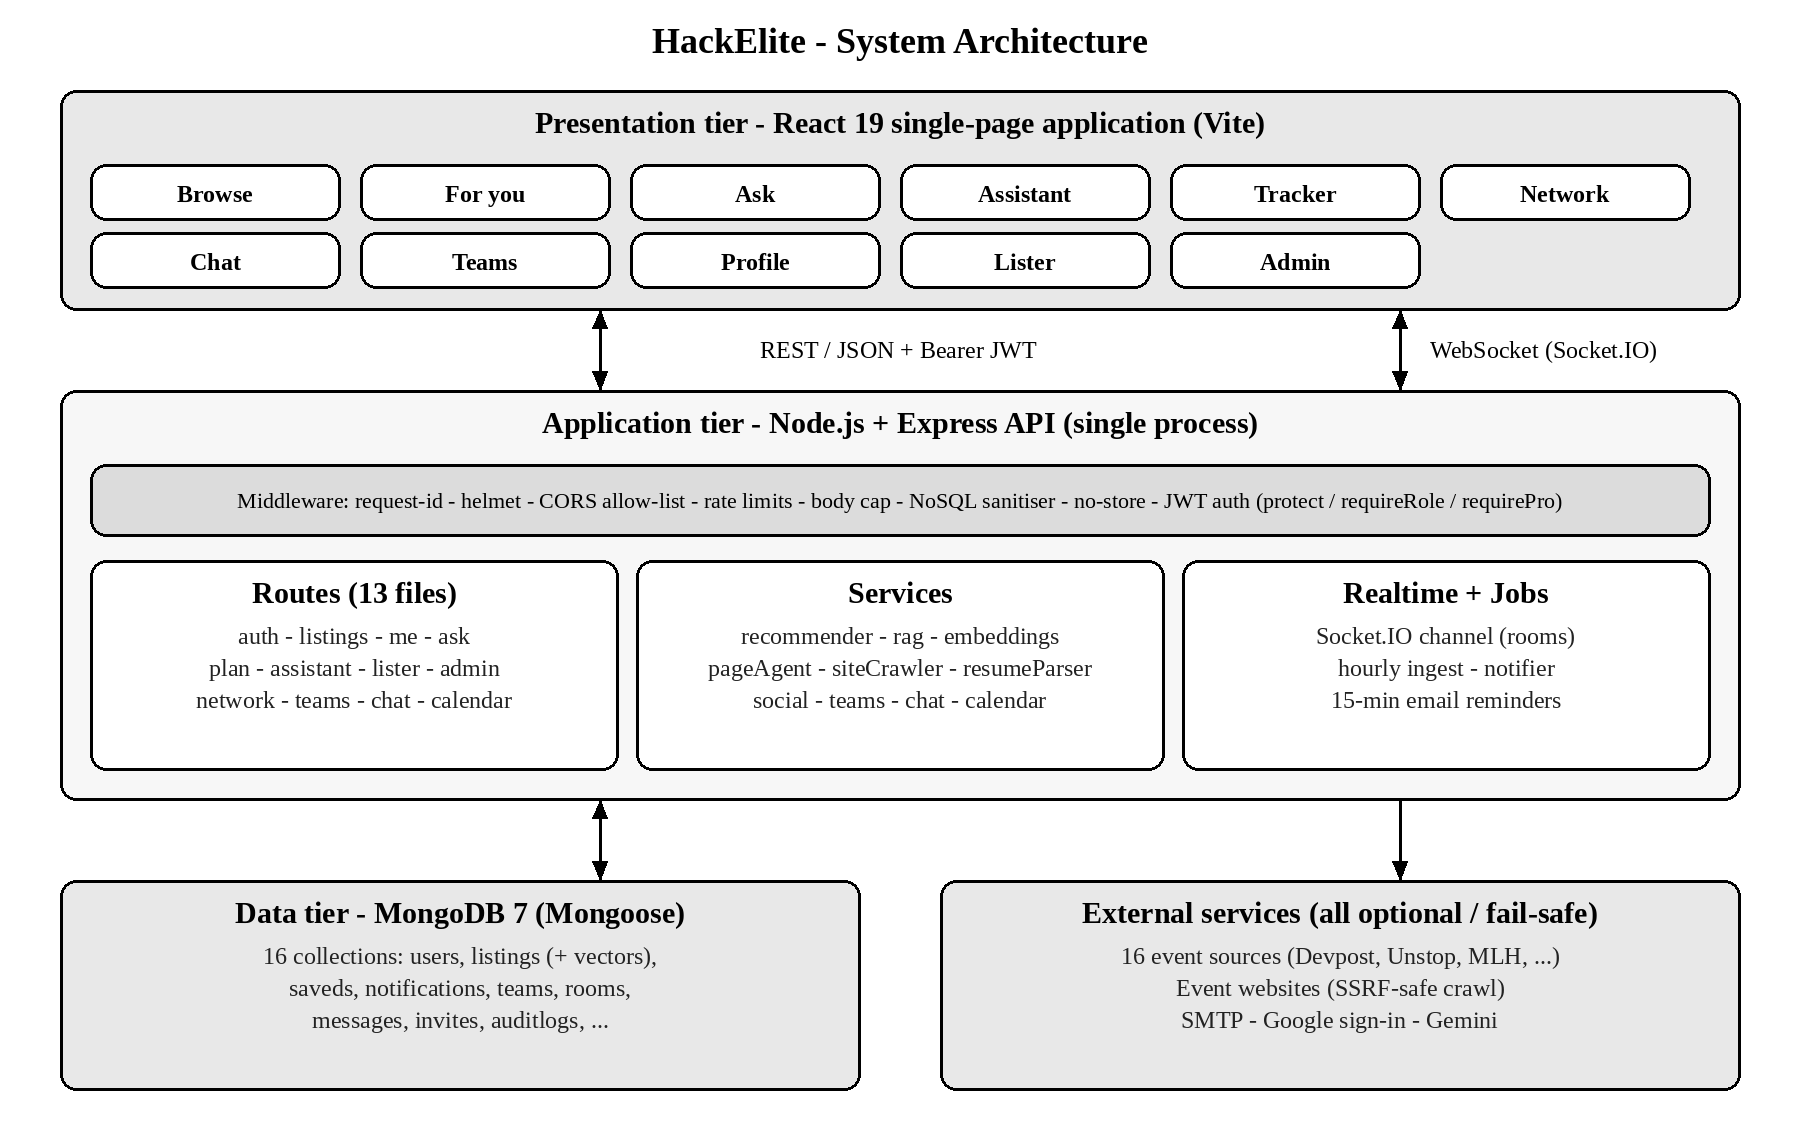
\includegraphics[width=0.95\textwidth]{images/system_architecture.png}
    \caption{System Architecture Diagram}
    \label{fig:system_architecture}
\end{figure}

\subsection{Request pipeline and authorisation}
Every HTTP request follows the same order: request identifier, security headers and CORS, rate limiting, compression, access log, \code{Cache-Control: private, no-store} for personalised routes, body parsing and sanitising, routers, and finally an error handler that never leaks stack traces. Authorisation is chained as \code{protect}, \code{requireRole}, \code{requirePro} and \code{requireApprovedLister}. The guiding principle is that authorisation is always enforced on the server and the client merely hides controls for convenience.

\subsection{Deployment architecture}
For production the Dockerfile builds the client in a first stage and ships one small non-root Node image that serves both API and client (\code{SERVE\_CLIENT=true}) under a hash-based content security policy. Docker Compose adds a MongoDB 7 container with a volume and a health-gated start. The Render blueprint deploys the same image with MongoDB Atlas, generates \code{JWT\_SECRET} and the Pro keys automatically, and uses \code{/api/health/ready} as its health check. The readiness probe returns 503 until MongoDB is connected, so an orchestrator only routes traffic to a working instance.

\section{Module Design}
The code base is organised into 13 route files, about 30 services (including 16 source adapters), 16 Mongoose models, three middleware files and a set of utilities, and a client with 17 pages. This section describes the main modules.

\subsection{Data model}
Figure~\ref{fig:er_diagram} shows the 16 collections and the main references between them. The \code{users} collection stores the email, bcrypt hash (excluded from queries by default), role, plan tier, profile, social settings and the parsed resume; resume text, chunk embeddings and the calendar token are excluded from every default query. The \code{listings} collection stores normalised event data, the numeric prize in rupees, the originating source and external identifier (unique together), the other sites on which the event also appears, and its embedding. Table~\ref{tab:collections} summarises each collection and its key indexes.

\begin{figure}[H]
    \centering
    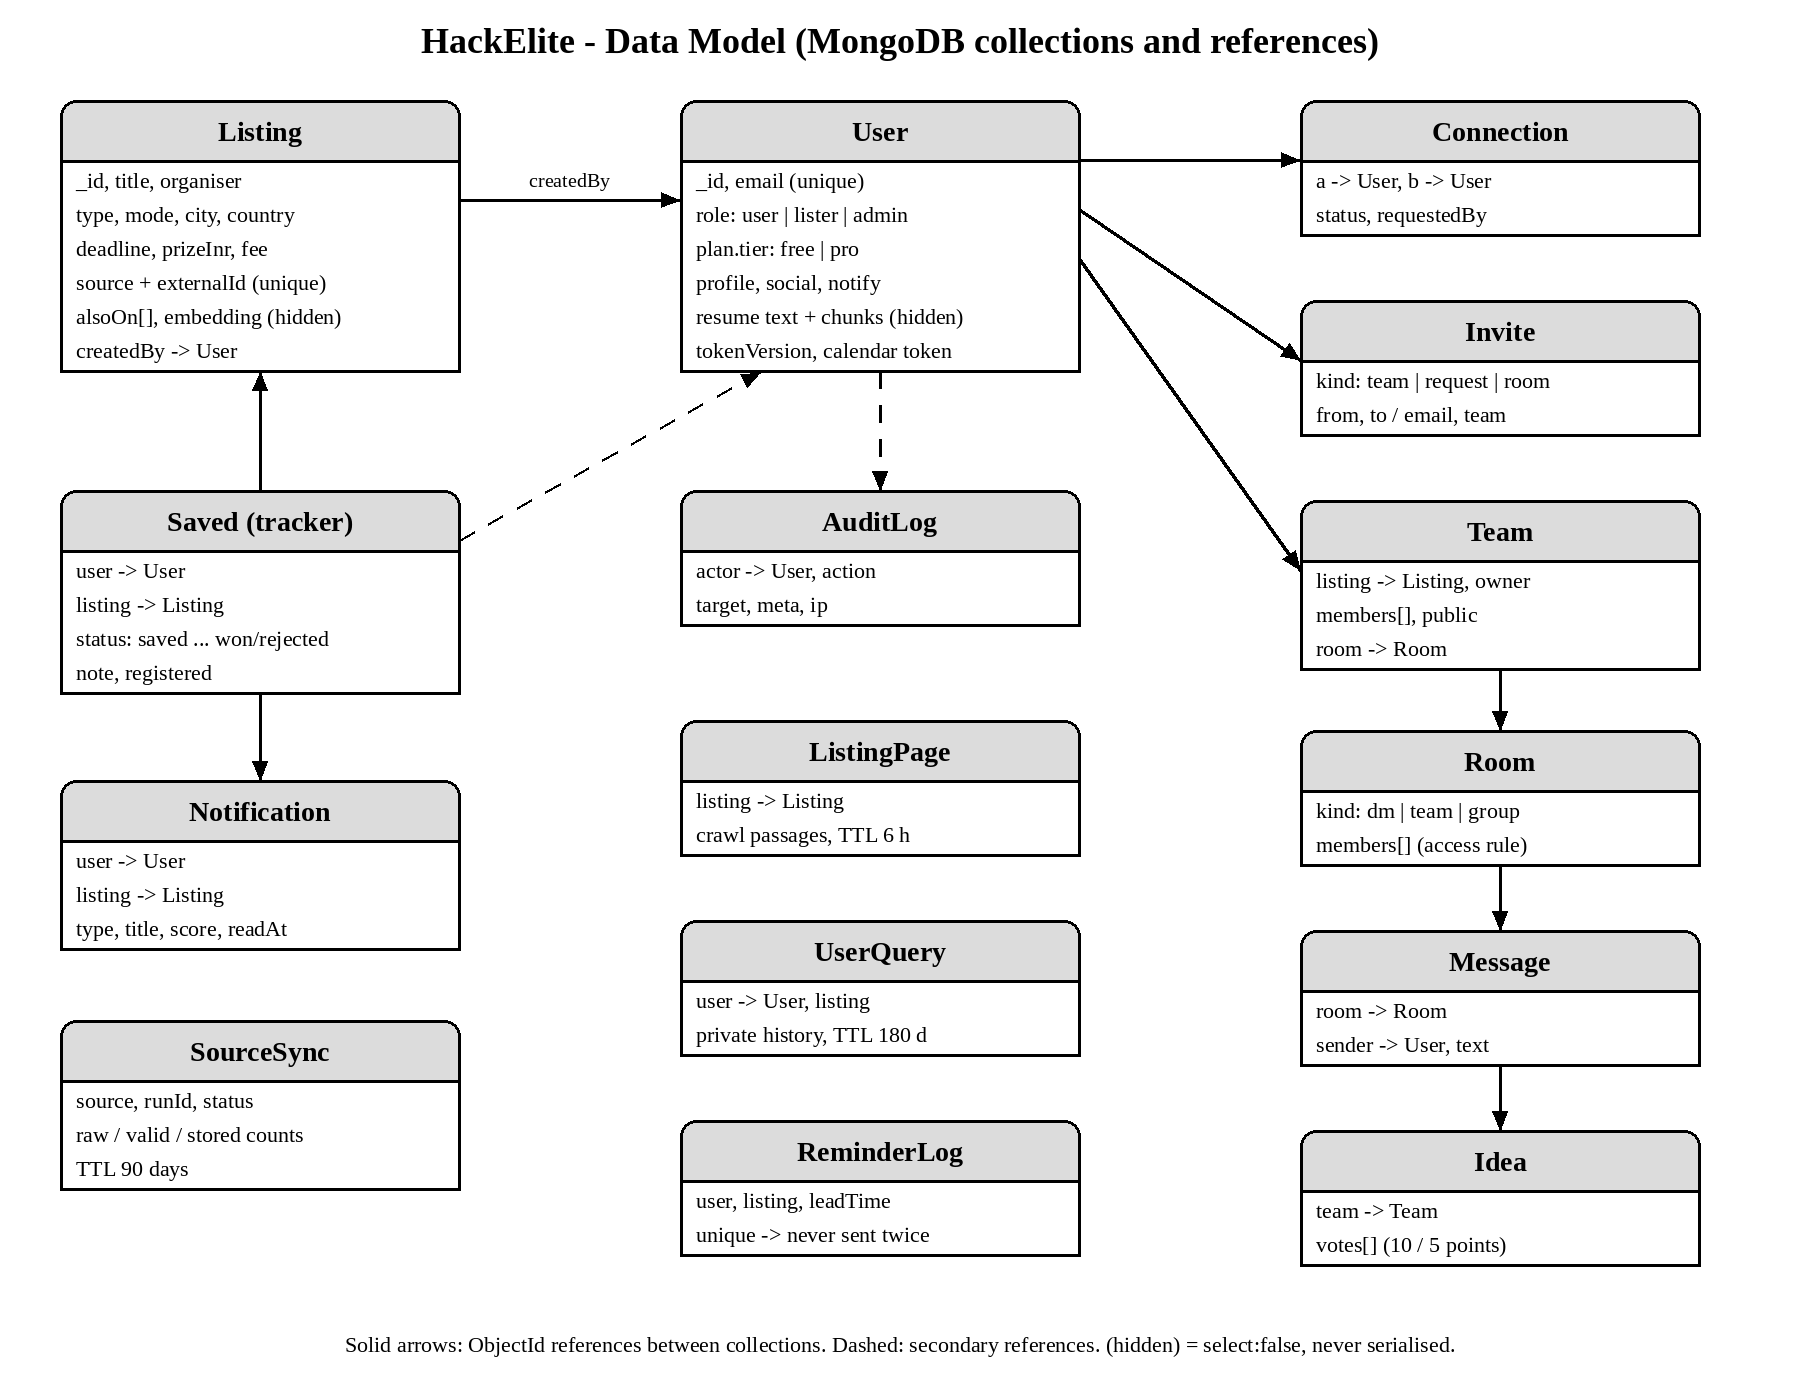
\includegraphics[width=0.95\textwidth]{images/er_diagram.png}
    \caption{Data Model: MongoDB Collections and References}
    \label{fig:er_diagram}
\end{figure}

\begin{table}[H]
\centering
\caption{MongoDB Collections and Key Indexes}
\label{tab:collections}
\small
\begin{tabularx}{\textwidth}{|>{\RaggedRight\arraybackslash}p{3cm}|X|X|}
\hline
\textbf{Collection} & \textbf{Purpose} & \textbf{Notable indexes / rules} \\
\hline
users & Accounts, roles, plan, profile, resume analysis, calendar token & email unique; googleId sparse unique; token version for revocation \\
\hline
listings & Normalised events with embeddings & (source, externalId) unique; (status, deadline); text index \\
\hline
sourcesyncs & One record per source per ingestion run & TTL 90 days \\
\hline
saveds & Tracker entries with status and note & (user, listing) unique \\
\hline
notifications & In-app alerts & (user, listing, type) unique, so reruns are idempotent \\
\hline
auditlogs & Security and administration events & createdAt, action \\
\hline
connections & Pairwise connection and block state & one document per user pair \\
\hline
invites & Team invites, join requests, room invites & shared accept pipeline \\
\hline
teams, rooms, messages & Teams, chat rooms (dm, team, group) and messages & membership is the only access rule \\
\hline
ideas & Team idea board with ranked votes & first choice 10 points, second 5 points \\
\hline
listingpages & Cache of crawled event pages & TTL 6 h on success, 10 min on failure \\
\hline
userqueries, listingquestions & Private question history and anonymous tally & TTL 180 days; no user id in the tally \\
\hline
reminderlogs & Record of reminders already sent & (user, listing, lead time) unique \\
\hline
\end{tabularx}
\end{table}

\subsection{Authentication and authorisation module}
Registration validates the password policy on the server and hashes the password with bcrypt at cost 12. A JWT with the user id and the user's \code{tokenVersion} (HS256, seven days) is issued. Changing the password, ``sign out everywhere'', disabling a user or changing a role increments \code{tokenVersion}, which invalidates all outstanding tokens and live sockets at once without a blacklist. Five failed logins lock the account for 15 minutes; unknown emails run a dummy bcrypt comparison so that timing and messages do not reveal which emails exist. Google sign-in verifies the signature, expiry, issuer, audience and \code{email\_verified} of the ID token on the server. Organisers who register are created in a pending state and notified administrators approve them before they can publish.

\subsection{Ingestion module}
Figure~\ref{fig:ingestion} shows the hourly ingestion pipeline. Each of the 16 adapters (Unstop, Devpost, Devfolio, HackerEarth, Codeforces, CodeChef, LeetCode, AtCoder, MLH, Hack Club, ETHGlobal, DoraHacks, GeeksforGeeks, Topcoder, Kaggle and clist) fetches raw records through a shared HTTP client that applies timeouts, retries with exponential back-off for network errors, 429 and 5xx responses, honours Retry-After, enforces a per-host delay and tracks pagination. The validator keeps, expires or rejects each record with a reason code. The de-duplicator merges records that share a canonical URL or the same normalised title and dates, preferring a native source over an aggregator and recording the other sites in an \code{alsoOn} list. The runner upserts primary records, moves users' tracker entries when a duplicate is merged, removes stale listings \emph{only} after a complete paginated sync, and writes a \code{SourceSync} record per source. The adapters run in parallel with \code{Promise.allSettled}, so one broken source never blocks another. Key-gated sources (Kaggle and clist) are reported as skipped when no key is configured.

\begin{figure}[H]
    \centering
    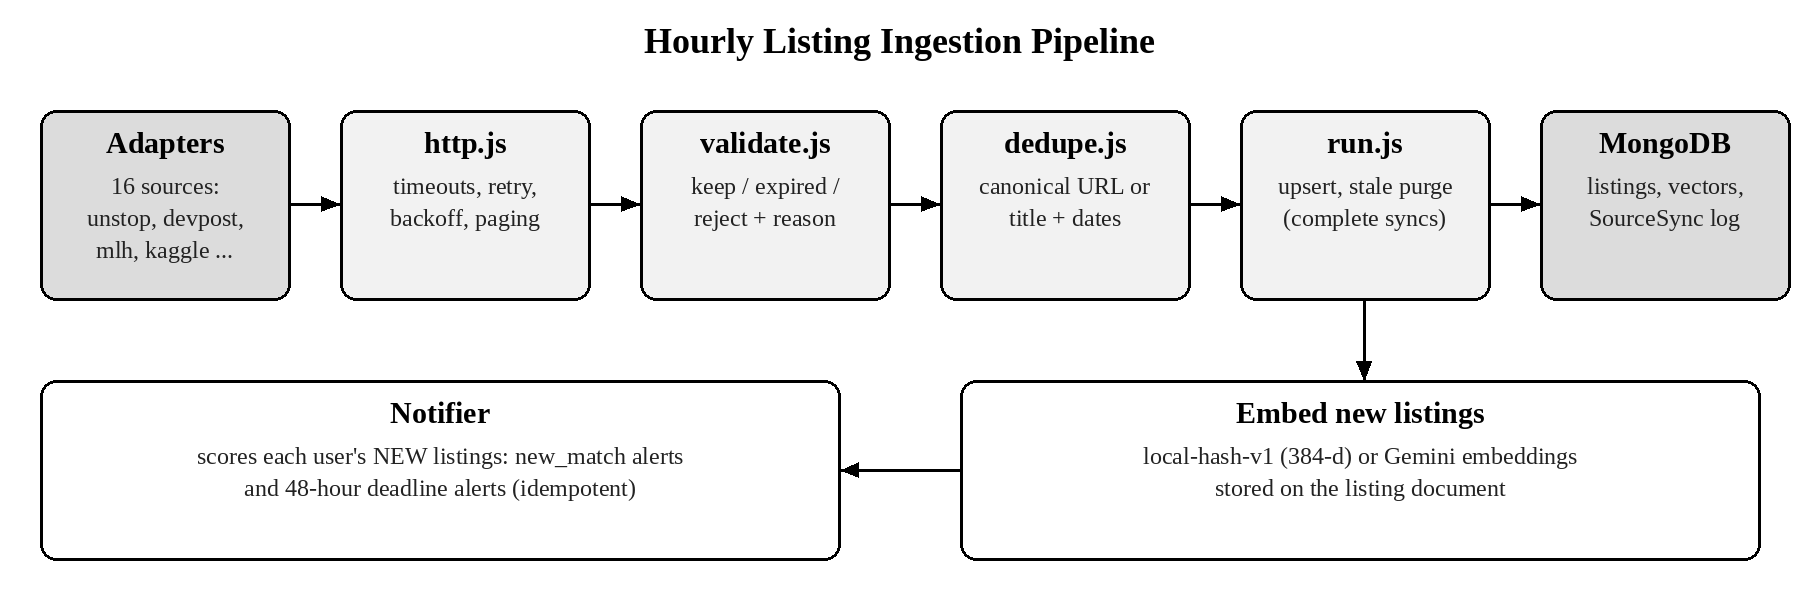
\includegraphics[width=0.95\textwidth]{images/ingestion_pipeline.png}
    \caption{Hourly Listing Ingestion Pipeline}
    \label{fig:ingestion}
\end{figure}

\subsection{Recommendation engine}
Figure~\ref{fig:recommender} summarises the recommender. Both tiers first apply hard filters that remove expired events, events the student is clearly not eligible for (education level or graduation batch), events already saved, and near-duplicates. The number excluded for each reason is returned to the client.

The \textbf{Free} score is $0.45 \times \text{interests} + 0.35 \times \text{skills} + 0.20 \times \text{urgency}$. The \textbf{Pro} score is the weighted sum of eight criteria given in Table~\ref{tab:rubric}, followed by multiplicative penalties: an in-person event abroad is multiplied by 0.5, an in-person event elsewhere for a student who does not travel by 0.75, an eligibility condition that cannot be verified by 0.9, and a paid event for a free-only student by 0.6. The result is an integer from 0 to 100 together with a list of criteria (label, weight, score, points and detail) and reasons in plain English. Ordering is deterministic (score, then deadline, then identifier), and skills are matched with a word-boundary dictionary so that \emph{Java} is not confused with \emph{JavaScript}. Location is resolved through an in-repository map of Indian cities and states, so no geocoding service is needed.

\begin{figure}[H]
    \centering
    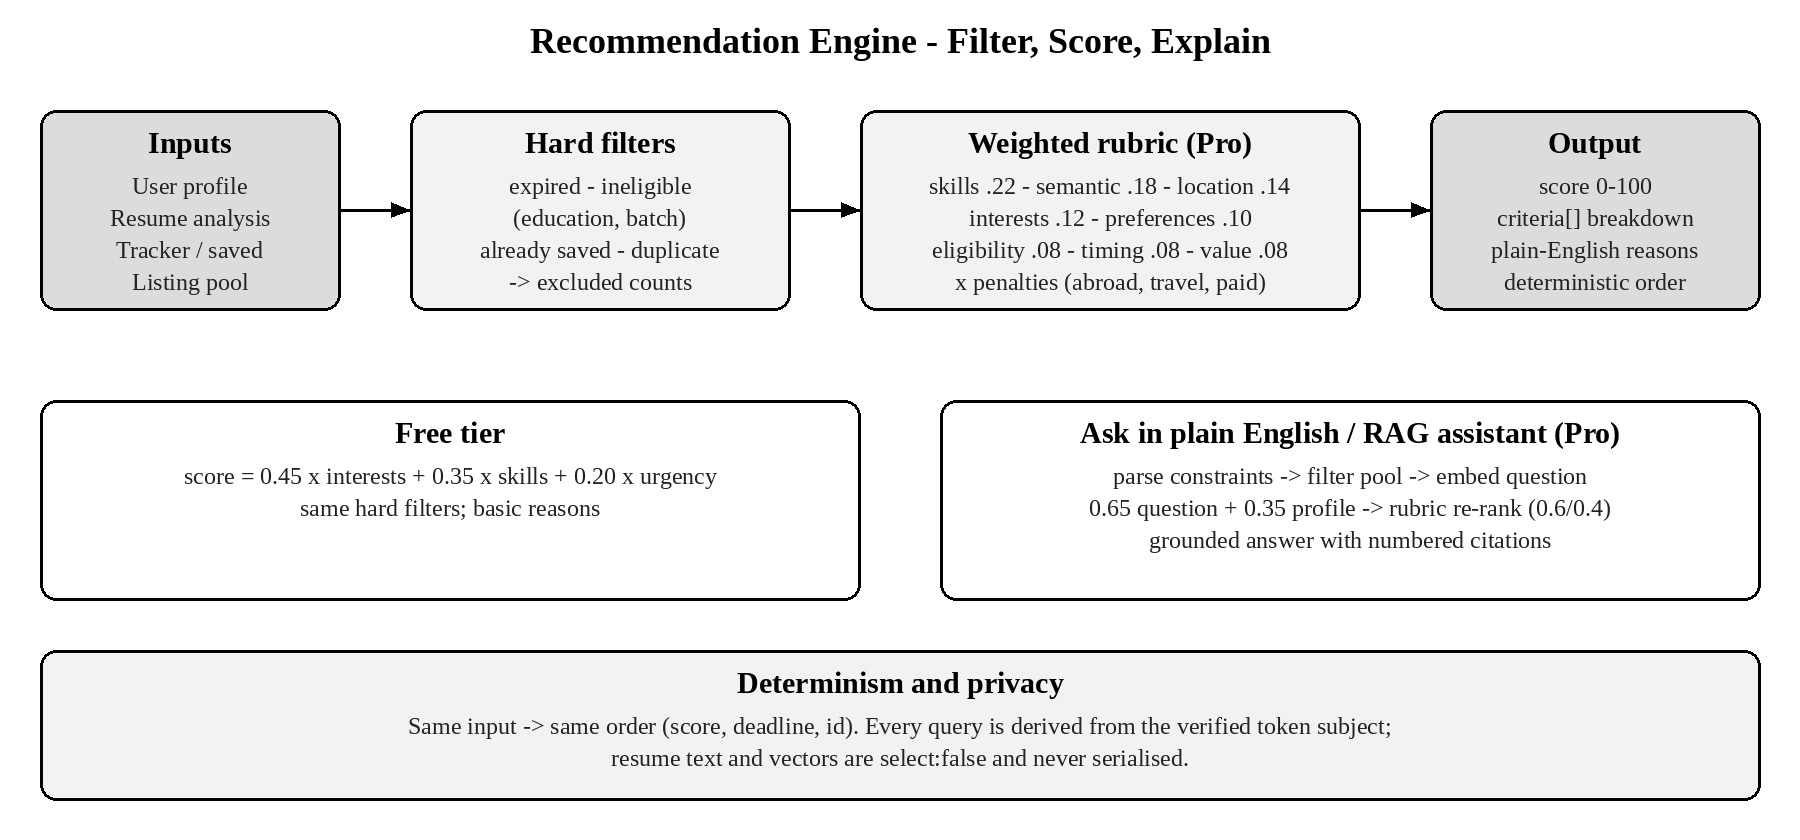
\includegraphics[width=0.95\textwidth]{images/recommendation_engine.png}
    \caption{Recommendation Engine: Filter, Score and Explain}
    \label{fig:recommender}
\end{figure}

\begin{table}[H]
\centering
\caption{Pro Recommendation Rubric}
\label{tab:rubric}
\begin{tabularx}{\textwidth}{|l|c|X|}
\hline
\textbf{Criterion} & \textbf{Weight} & \textbf{What it measures} \\
\hline
Skills & 0.22 & Overlap between resume/profile skills and the event's required or tagged skills \\
\hline
Semantic fit & 0.18 & Cosine similarity between the profile/resume vectors and the event vector \\
\hline
Location & 0.14 & Online, same city or state, travel willingness, country-aware \\
\hline
Interests & 0.12 & Match between interests (inferred or entered) and event themes \\
\hline
Preferences & 0.10 & Event type, fee and mode preferences \\
\hline
Eligibility & 0.08 & Education level and graduation batch \\
\hline
Timing & 0.08 & Time left before the deadline relative to effort needed \\
\hline
Prize value & 0.08 & Prize against expected competition \\
\hline
\end{tabularx}
\end{table}

\subsection{Resume Studio and parsing module}
The resume parser accepts PDF, DOCX or TXT files up to 5 MB. It checks the extension and the file's magic bytes (a fake \code{.pdf} is rejected), parses the document in memory with \code{pdf-parse} or \code{mammoth}, and never writes the file to disk. It extracts skills from a dictionary of about 50 canonical skills with aliases, infers interests with scores, and estimates the graduation year. The text is split into at most 20 overlapping chunks of 650 characters and each chunk is embedded for later retrieval. All resume text and vectors are stored with \code{select:false} and are never serialised to any client.

\subsection{Embeddings and retrieval-augmented assistant}
Embeddings use \code{local-hash-v1}, a deterministic 384-dimensional feature-hashing model over words, bigrams and canonical skill tokens that needs no network, or optionally Gemini \code{gemini-embedding-001} truncated to 768 dimensions. Vectors of different models are never compared; switching the model re-indexes lazily. For the assistant, the question is first parsed for hard constraints (type, mode, closing window, prize and fee) that filter the candidate pool. The question is embedded, candidates are scored as $0.65 \times \text{question similarity} + 0.35 \times \text{profile similarity}$, re-ranked as $0.6 \times \text{relevance} + 0.4 \times \text{rubric}$, and the two best resume chunks are added. A grounded prompt with numbered context is sent to Gemini when a key exists; otherwise an extractive answer is assembled from the top matches. Listing text is treated as untrusted data, and responses always carry citations.

\subsection{Per-event agent and site crawler}
Figure~\ref{fig:agent} shows how a question about a single event is answered. The server reads the event's own URL through \code{safeFetch}, which accepts only http and https on ports 80 and 443, resolves the host itself, requires every address to be public (loopback, private, link-local, carrier-grade NAT, cloud-metadata and IPv6 including IPv4-mapped addresses are refused), pins the connection to the vetted address to defeat DNS rebinding, revalidates each redirect (at most four), and limits time, size and content type. The crawler honours \code{robots.txt} and Crawl-delay, issues at most one request per second to a host, follows up to six same-host links to official pages such as FAQ, rules and schedule, and never fetches forums, participant pages or other user-generated areas. Passages are extracted with cheerio (scripts, navigation and forms removed; headings, paragraphs, list items, table cells, meta description and schema.org \code{Event} data kept), combined with one passage per stored fact of the listing, and retrieved using embeddings, question-word coverage and an intent boost. Answers cite their sources and say honestly when a page cannot be read, for example when it renders only with JavaScript. Crawled passages are cached in MongoDB for six hours.

\begin{figure}[H]
    \centering
    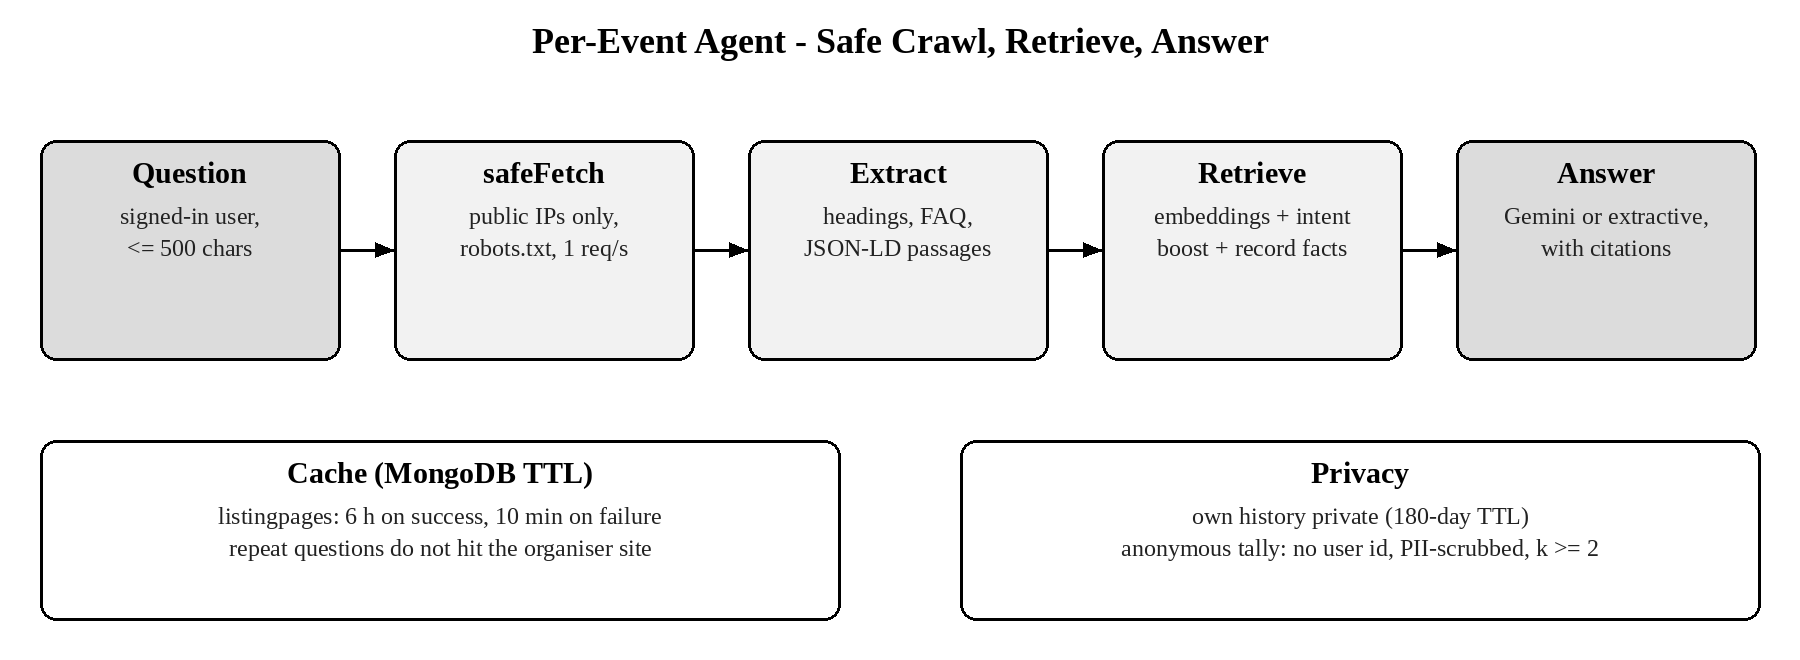
\includegraphics[width=0.95\textwidth]{images/agent_flow.png}
    \caption{Per-Event Agent: Safe Crawl, Retrieve and Answer}
    \label{fig:agent}
\end{figure}

\subsection{Network, teams, chat and reminders}
A \code{Connection} document represents the relationship between two users; a shared \code{Invite} pipeline handles team invitations, join requests and room invitations. A \code{Room} (direct message, team or group) is accessible only to its members, and non-members receive the same 404 response for a room that is not theirs and one that does not exist. Sockets are joined to rooms by the server from the database, never at the client's request, and a socket is dropped immediately when the session is revoked. Discovery is opt-in (default off), only name, headline and skills are shown, and email addresses are never returned. The Free versus Pro split (Table~\ref{tab:plans}) is checked inside the services, so no route can bypass it. The reminder scheduler runs every 15 minutes, sends at most one email per user, event and lead time (recorded in \code{ReminderLog}), and never after the deadline.

\begin{table}[H]
\centering
\caption{Free versus Pro Plan}
\label{tab:plans}
\small
\begin{tabularx}{\textwidth}{|X|c|c|}
\hline
\textbf{Capability} & \textbf{Free} & \textbf{Pro} \\
\hline
Browse, search, filter, expand cards, plain-English Ask & Yes & Yes \\
\hline
Tracker, notifications, email reminders, calendar links and live feed & Yes & Yes \\
\hline
Per-event agent, connections, live direct messages, joining invited teams & Yes & Yes \\
\hline
Basic picks from skills and interests & Yes & Yes \\
\hline
Resume upload and analysis & No & Yes \\
\hline
Full eight-criterion recommendations with explanations & No & Yes \\
\hline
Retrieval-augmented assistant with citations & No & Yes \\
\hline
Host teams and private rooms, invite people, Team up button & No & Yes \\
\hline
Teammate and open-team recommendations, people search, public teams, idea voting & No & Yes \\
\hline
\end{tabularx}
\end{table}

\subsection{Calendar module}
The calendar builder produces RFC 5545 output with UTC times, correct text escaping, line folding at 75 octets without splitting UTF-8 characters, stable UIDs (\code{deadline-\textless id\textgreater} and \code{event-\textless id\textgreater}) and a SEQUENCE derived from the listing's update time, so that calendar applications update an event in place instead of duplicating it. For each listing the system provides Google, Outlook.com and Microsoft 365 add-event links and a downloadable \code{.ics} file. A personal live feed is a capability URL protected by a 192-bit random token that can be rotated or revoked; it contains the tracker (except rejected items) and, optionally, top picks, with reminders chosen by the user, and never includes notes.

\subsection{Security design}
Table~\ref{tab:security} lists the principal controls. Each control is covered by an automated test; the repository also keeps an honest list of known gaps.

\begin{table}[H]
\centering
\caption{Principal Security Controls}
\label{tab:security}
\small
\begin{tabularx}{\textwidth}{|l|X|}
\hline
\textbf{Area} & \textbf{Control} \\
\hline
Passwords & Policy of 10 or more characters with four classes; bcrypt cost 12; breached-password check using k-anonymity (only a 5-character SHA-1 prefix leaves the server) \\
\hline
Brute force & Five failures lock the account for 15 minutes; auth endpoints limited to 30 requests per 15 minutes per IP; identical errors for unknown and wrong credentials \\
\hline
Sessions & HS256 JWT with pinned algorithm and \code{tokenVersion} for instant revocation of tokens and sockets \\
\hline
Authorisation & Server-side role, plan and ownership checks; mass-assignment whitelist; admin bootstrap only from environment \\
\hline
Injection & Stripping of keys beginning with \code{\$}, dotted keys and \code{\_\_proto\_\_}; regex input escaped; strict Mongoose schemas \\
\hline
Transport & helmet (CSP, nosniff, frame-ancestors none, HSTS in production); CORS allow-list with no wildcard \\
\hline
Abuse limits & 300 requests per minute globally; 20 per minute on heavy endpoints; 200 KB JSON and 5 MB upload caps \\
\hline
Uploads & Extension allow-list and magic-byte check; parsed in memory only \\
\hline
SSRF-safe crawling & Public addresses only, connection pinning, redirect revalidation, size and time caps, robots.txt honoured \\
\hline
Realtime & Handshake requires a valid JWT for an active user; server-decided rooms; 20 messages per 10 s per socket; 16 KB payload cap \\
\hline
Privacy & \code{no-store} on personal routes; resume text and vectors never serialised; opt-in discovery; anonymous question tally with k $\ge$ 2; full account erasure \\
\hline
Audit & Registration, login, lockout, plan, role and listing changes, and deletions are recorded \\
\hline
\end{tabularx}
\end{table}

\subsection{Client design}
The client is a React 19 single-page application with a sticky header, a hero section showing live statistics, a filter bar and a card grid. Pages are Home/Browse, For you, Ask, Assistant, Tracker, Network, Chat, Teams, Team room, Profile, Listing detail, Notifications, Plan, Lister dashboard, Admin and Auth. State that must be shared (authentication, toasts, realtime connection) lives in React context providers; API access is centralised in one module that attaches the bearer token and handles errors uniformly. The interface supports a light and a dark theme, honours the reduced-motion preference, and uses skeleton, empty and error states.

% ---------------- Chapter 4 ----------------
\chapter{IMPLEMENTATION AND RESULTS}

\section{Implementation Overview}
The project was implemented iteratively. The first version (kept in the \code{old/} directory of the repository for reference) offered browsing and basic applications. It was then re-architected into the current platform in the following stages: (1) a secure foundation with authentication, roles and configuration validation; (2) the ingestion pipeline and listing model; (3) the recommender, resume parser and embeddings; (4) the assistant, per-event agent and crawler; (5) tracker, notifications and calendar integration; (6) network, teams, chat and reminders; (7) the redesigned user interface; and (8) deployment, continuous integration, the live end-to-end journey and documentation.

\subsection{Technology and size}
The server consists of about 9,600 lines of JavaScript (routes, services, models, middleware, utilities and scripts), the client of about 5,100 lines of JavaScript, JSX and CSS, and the automated tests of about 2,800 lines. The server is started with \code{node server.js}; in development a single command, \code{npm run dev}, starts a real local MongoDB, the API on port 5050 and the Vite development server on port 5173. Table~\ref{tab:commands} lists the principal commands.

\begin{table}[H]
\centering
\caption{Principal Project Commands}
\label{tab:commands}
\small
\begin{tabularx}{\textwidth}{|l|X|}
\hline
\textbf{Command} & \textbf{Purpose} \\
\hline
\code{npm run setup} & Install server and client dependencies \\
\hline
\code{npm run dev} & Start MongoDB, API and web client with hot reload \\
\hline
\code{npm test} & Run the 114 unit, integration and in-process journey tests \\
\hline
\code{npm run e2e} & Boot the real server process and run the 41-check live journey \\
\hline
\code{npm run verify} & Tests, client build and live end-to-end run (merge gate) \\
\hline
\code{npm run ingest} & Refresh listings from all sources \\
\hline
\code{npm run sources:check} & Probe each of the 16 adapters against its live site \\
\hline
\code{npm run docker:up} & Run the application and MongoDB in containers \\
\hline
\end{tabularx}
\end{table}

\subsection{REST API and real-time protocol}
The API exposes more than 100 HTTP routes, grouped into 13 routers as summarised in Table~\ref{tab:api}. Every personalised route requires sign-in and sends \code{Cache-Control: private, no-store}. The WebSocket protocol uses the same JWT in the handshake. The client sends \code{message:send} (with acknowledgement), \code{typing} and \code{room:read}; the server sends \code{message:new}, \code{typing}, \code{notification:new}, \code{room:added}, \code{room:removed} and \code{ready}. A REST endpoint for sending messages is a full fallback when a WebSocket cannot be used.

\begin{table}[H]
\centering
\caption{REST API Route Groups}
\label{tab:api}
\small
\begin{tabularx}{\textwidth}{|l|l|X|}
\hline
\textbf{Router} & \textbf{Base path} & \textbf{Responsibility} \\
\hline
auth & \code{/api/auth} & Register, login, Google, logout, password change and reset, verification, account deletion \\
\hline
listings & \code{/api/listings} & Public catalogue, search, filters, statistics, detail \\
\hline
me & \code{/api/me} & Profile, resume, recommendations, tracker, notification settings \\
\hline
ask / assistant & \code{/api/ask}, \code{/api/assistant} & Plain-English search and the Pro retrieval-augmented assistant \\
\hline
listingAgent & \code{/api/listings/:id/ask} & Per-event agent, history and question tally \\
\hline
plan & \code{/api/plan} & Plan status and Pro activation \\
\hline
calendar & \code{/api/calendar} & Add-event links, \code{.ics} files, feed token and live feed \\
\hline
network & \code{/api/network} & Connections, people search, requests, invites, recommendations \\
\hline
teams & \code{/api/teams} & Teams, invites, join requests, ideas and votes \\
\hline
chat & \code{/api/chat} & Rooms, messages, read state, room invites \\
\hline
lister & \code{/api/lister} & Organiser listings and question insights \\
\hline
admin & \code{/api/admin} & Users, listers, listings, sources, integrations and audit log \\
\hline
\end{tabularx}
\end{table}

\subsection{Sources and ingestion results}
Table~\ref{tab:sources} lists the 16 adapters and their interfaces. Records are normalised to a common schema; dates are converted to UTC with the correct source time zone (for example IST for Unstop, Eastern time for Devpost and JST for AtCoder), and prizes are parsed with currency (USD, INR, EUR and others, with K, L, Cr and M suffixes) and converted to an approximate rupee value while the original amount is always shown. A live run populated about 940 open listings from 10 sources, with the remainder skipped because they need keys or sit behind bot verification.

\begin{table}[H]
\centering
\caption{Listing Sources}
\label{tab:sources}
\small
\begin{tabularx}{\textwidth}{|l|X|l|}
\hline
\textbf{Source} & \textbf{Interface used} & \textbf{Key needed} \\
\hline
Unstop & Public JSON search API (hackathons, competitions, quizzes) & No \\
\hline
Devpost & Public JSON hackathons API & No \\
\hline
Devfolio & Public JSON API (open and upcoming) & No \\
\hline
HackerEarth & JSON feed & No \\
\hline
Codeforces, AtCoder & Official contest list / contest page & No \\
\hline
CodeChef, LeetCode & Public contest endpoints & No \\
\hline
MLH, GeeksforGeeks & HTML with microdata or embedded data & No \\
\hline
ETHGlobal & Embedded Next.js data & No \\
\hline
Hack Club, Topcoder & Public feeds / API & No \\
\hline
DoraHacks & Bot-protected; skipped unless an authorised endpoint is configured & Optional URL \\
\hline
Kaggle, clist & Official APIs & Yes (free) \\
\hline
\end{tabularx}
\end{table}

\section{Result Snapshots}
This section presents the running application. The listings shown are live data ingested from the public sources.

Figure~\ref{fig:home} shows the home page. A hero section states the proposition, live statistics (open listings, closing in seven days, total prize money listed and platform count) are computed from the database, and a filter bar supports search, type, platform, mode, soonest deadline, free entry and closing this week. Cards show the days left, type, mode, city, prize, fee and team size.

\begin{figure}[H]
    \centering
    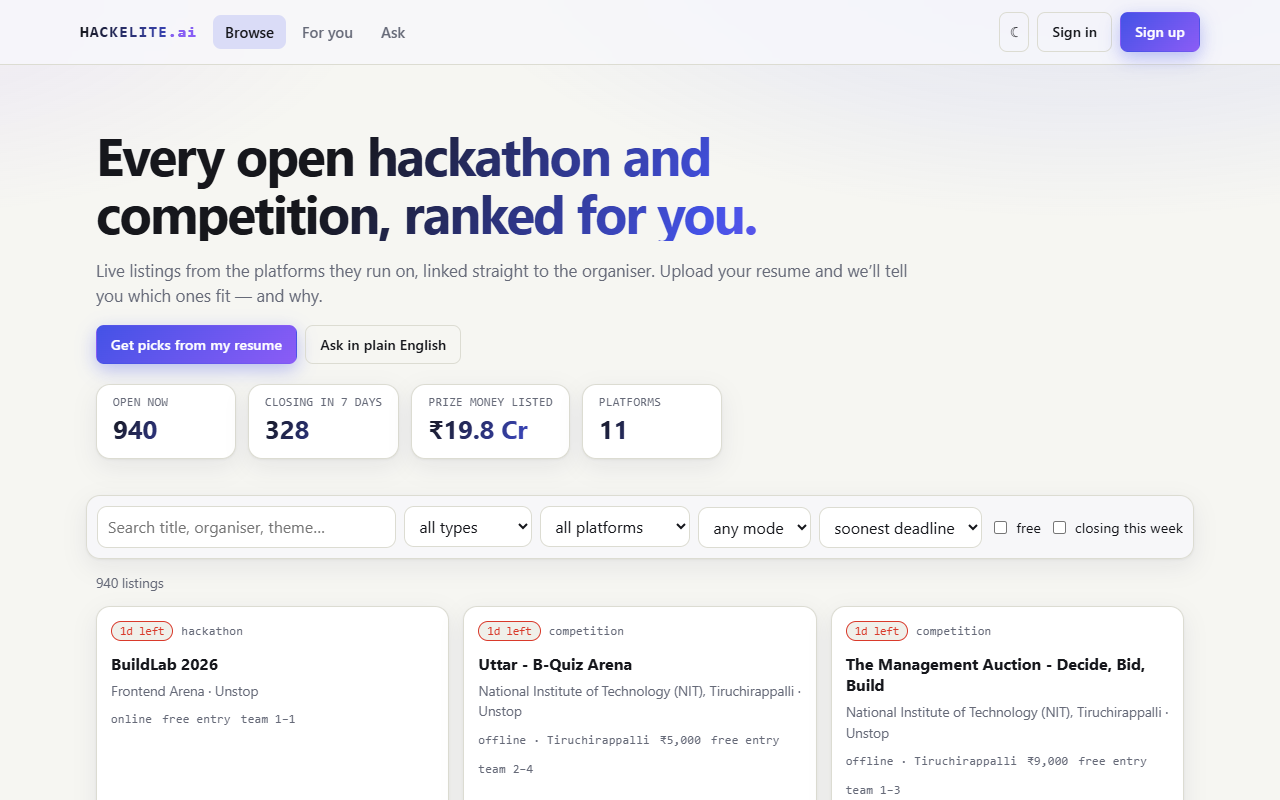
\includegraphics[width=0.92\textwidth]{images/home.png}
    \caption{Home Page with Live Statistics, Filters and Event Cards}
    \label{fig:home}
\end{figure}

Clicking a card expands it in place and shows every detail, with a Register link to the organiser (Figure~\ref{fig:card}). Registering saves the event to the tracker as \emph{applied}.

\begin{figure}[H]
    \centering
    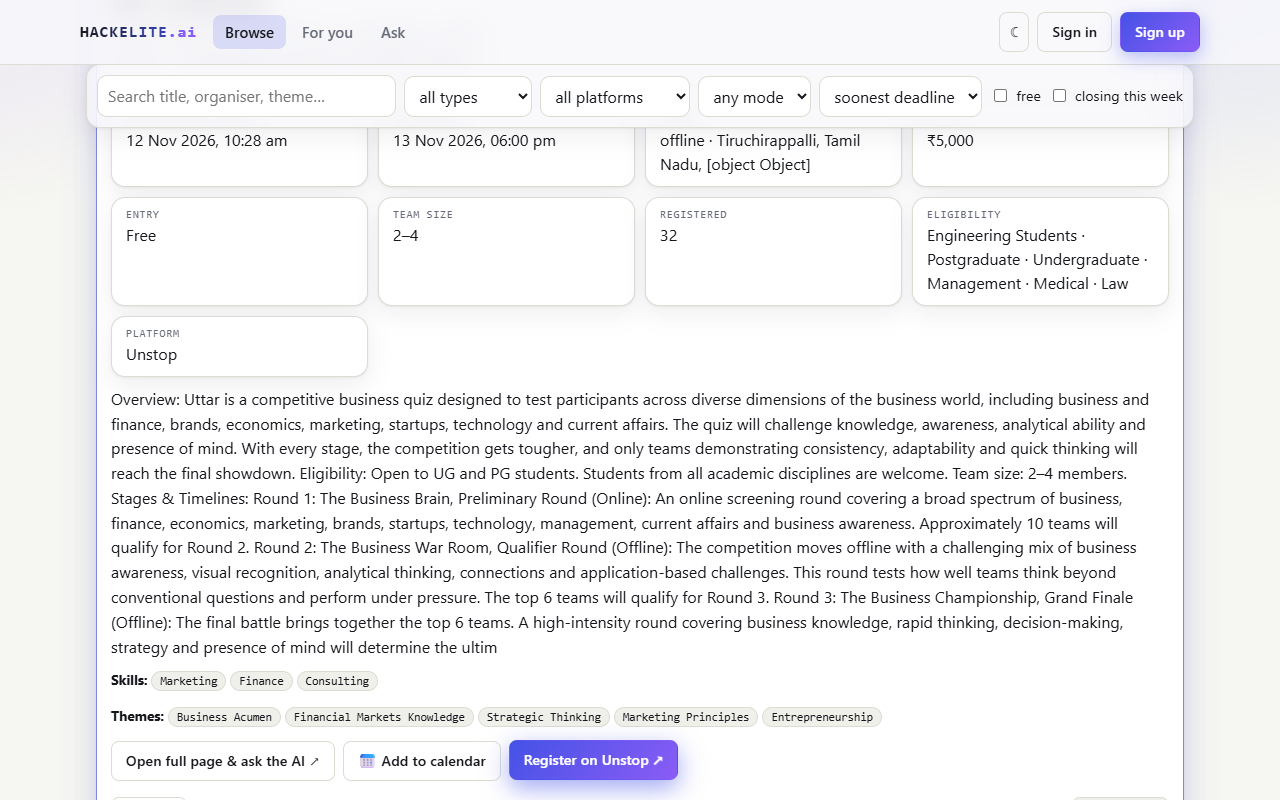
\includegraphics[width=0.92\textwidth]{images/card-expanded.png}
    \caption{Expanded Event Card}
    \label{fig:card}
\end{figure}

The For you page combines Resume Studio and the explainable picks (Figure~\ref{fig:foryou}). A dropped PDF or DOCX is parsed in memory; skills, interests and the graduation year are shown, and the ranked picks refresh immediately with score breakdowns.

\begin{figure}[H]
    \centering
    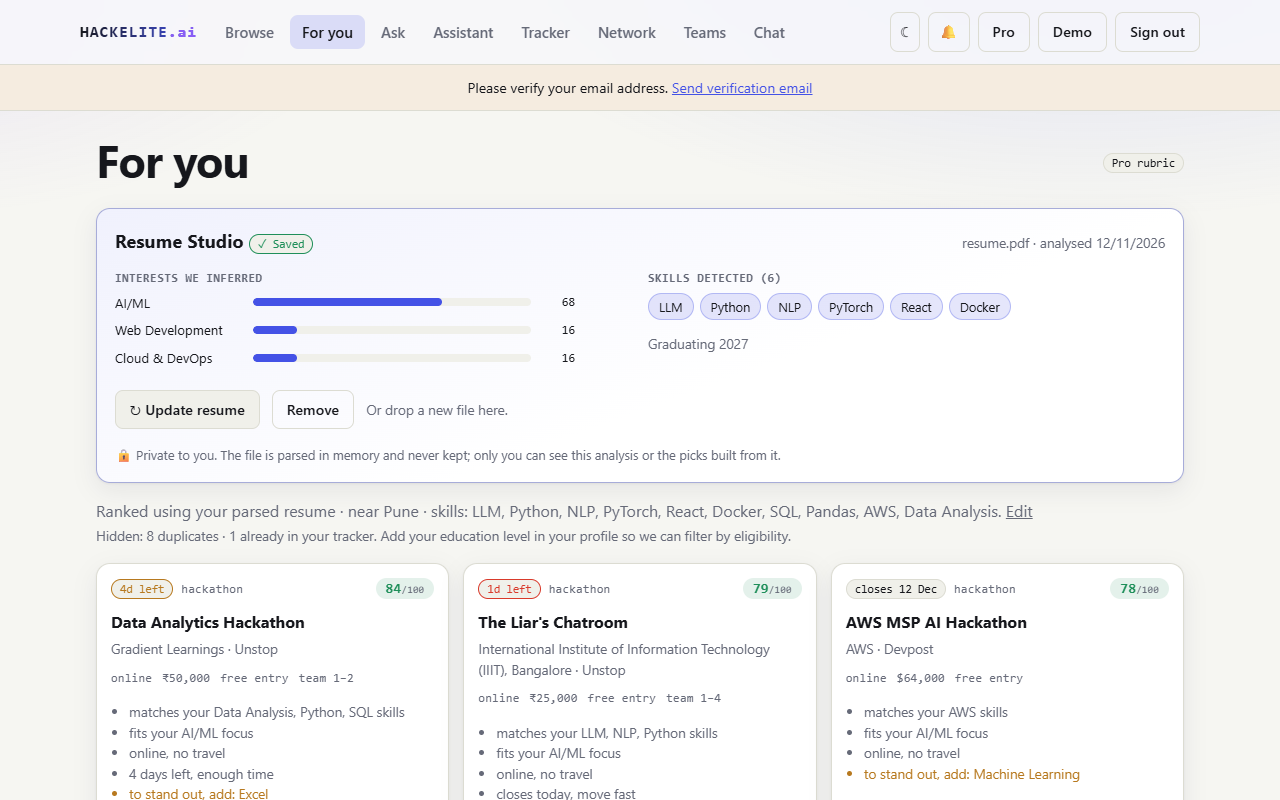
\includegraphics[width=0.92\textwidth]{images/for-you-resume-studio.png}
    \caption{Resume Studio and Explainable Recommendations}
    \label{fig:foryou}
\end{figure}

On every listing page the ``Ask this hackathon'' agent answers questions from the event's own website and shows its sources (Figure~\ref{fig:agentui}).

\begin{figure}[H]
    \centering
    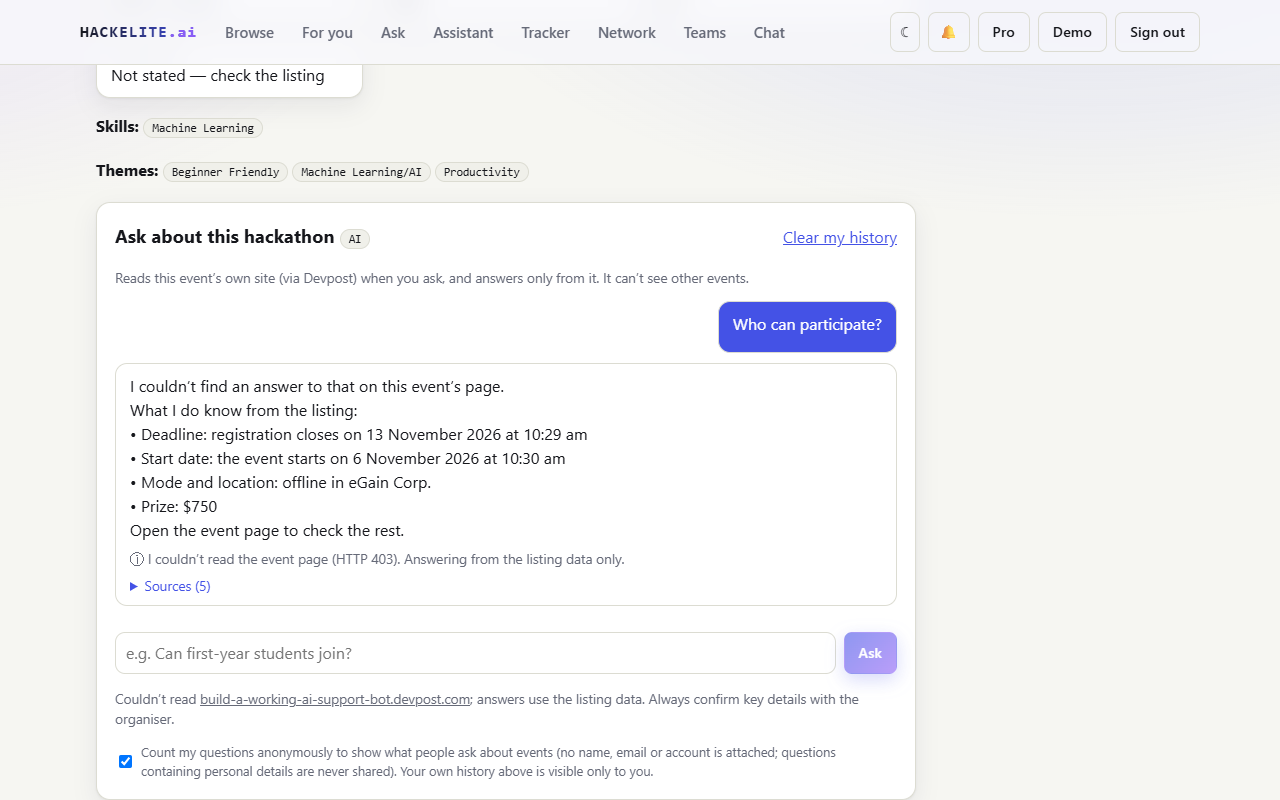
\includegraphics[width=0.92\textwidth]{images/listing-agent.png}
    \caption{Per-Event Agent Answering with Cited Sources}
    \label{fig:agentui}
\end{figure}

The tracker lists saved and applied events with status and notes, and the sync panel provides add-to-calendar links and a live private feed (Figure~\ref{fig:tracker}).

\begin{figure}[H]
    \centering
    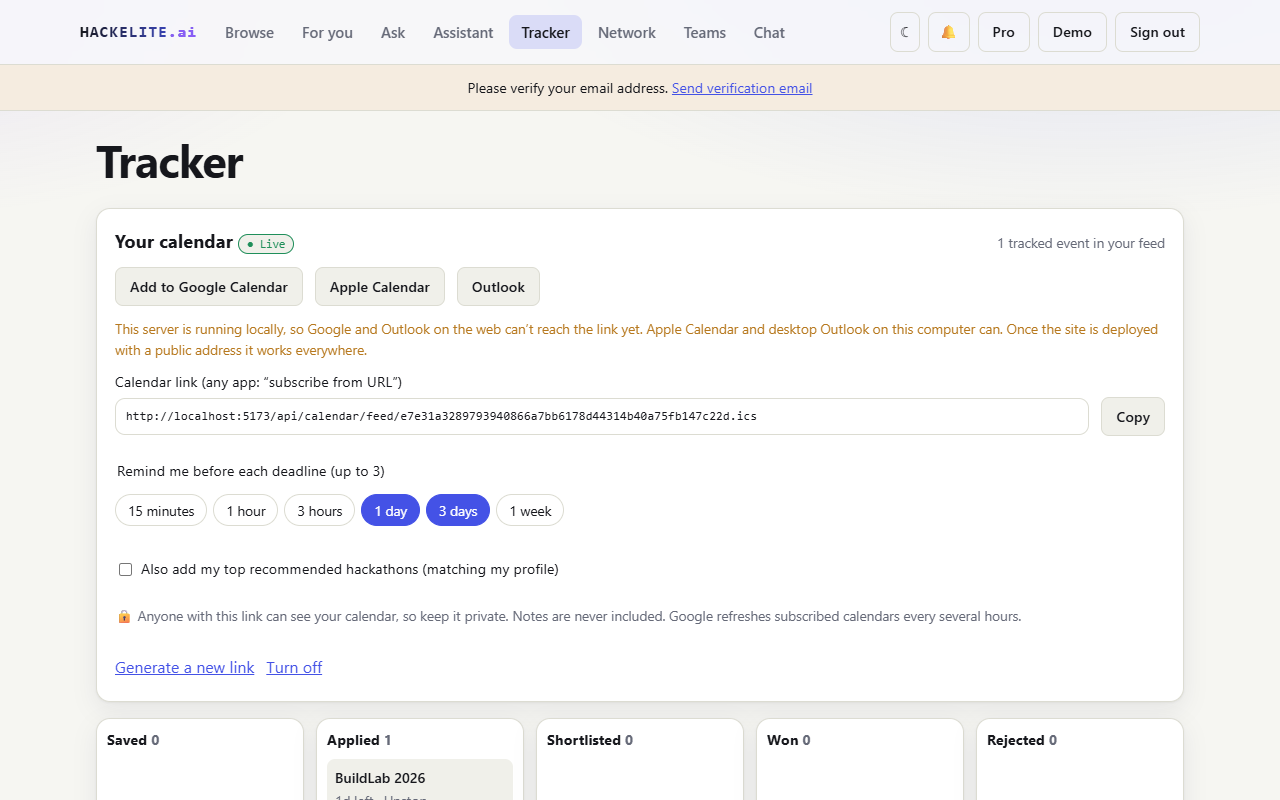
\includegraphics[width=0.92\textwidth]{images/tracker-calendar.png}
    \caption{Tracker and Live Calendar Sync}
    \label{fig:tracker}
\end{figure}

The Network page shows pending requests, people who opted in to discovery and suggestions (Figure~\ref{fig:network}); the Chat page provides live private conversations with unread badges (Figure~\ref{fig:chat}).

\begin{figure}[H]
    \centering
    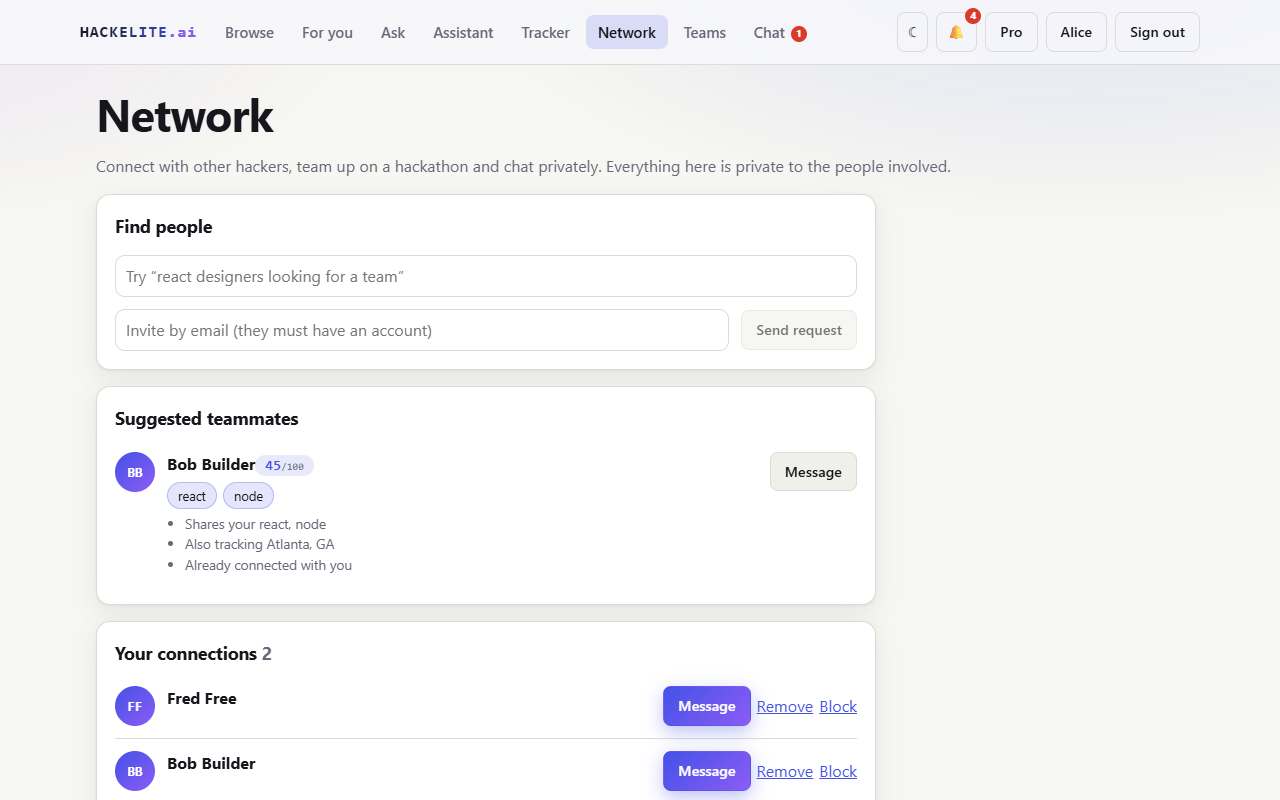
\includegraphics[width=0.92\textwidth]{images/network.png}
    \caption{Network: Requests, People and Suggestions}
    \label{fig:network}
\end{figure}

\begin{figure}[H]
    \centering
    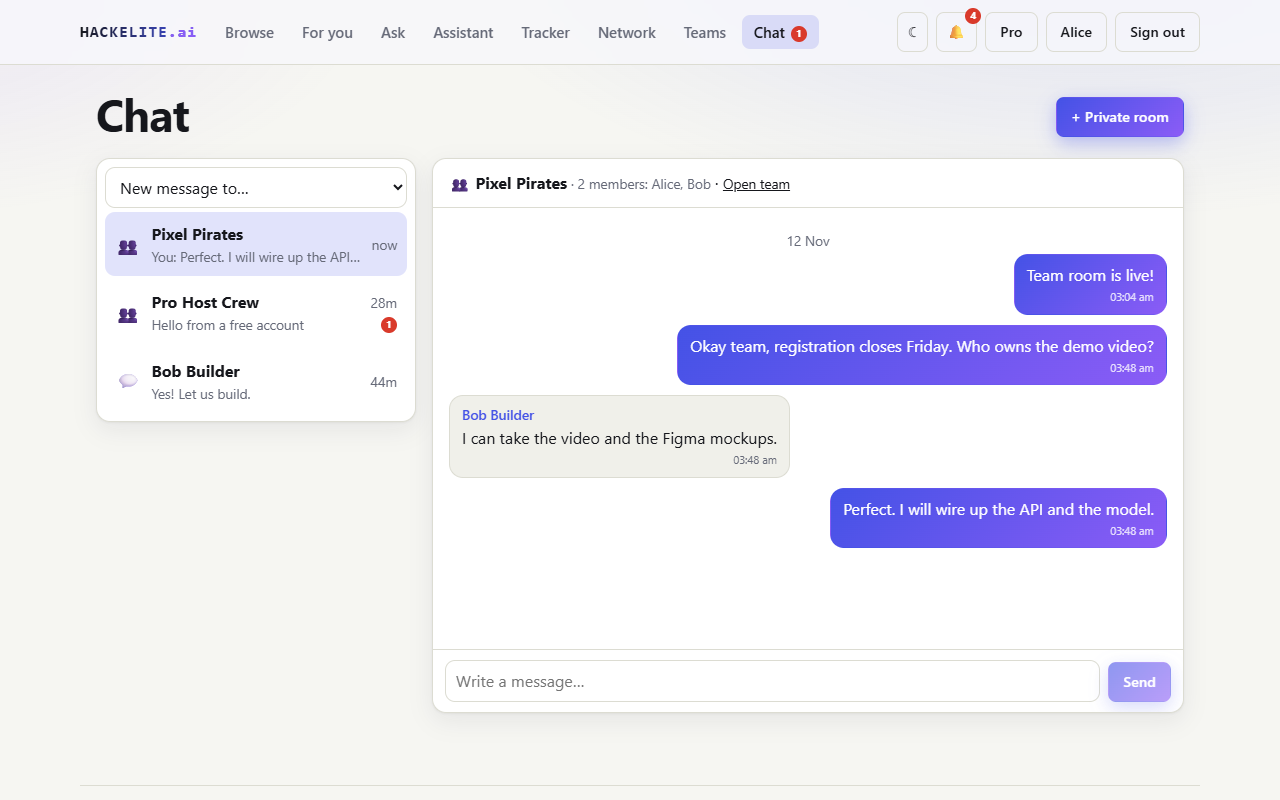
\includegraphics[width=0.92\textwidth]{images/chat.png}
    \caption{Live Private Chat}
    \label{fig:chat}
\end{figure}

A team room combines membership, invitations, the linked hackathon and the idea board with ranked voting (Figure~\ref{fig:team}).

\begin{figure}[H]
    \centering
    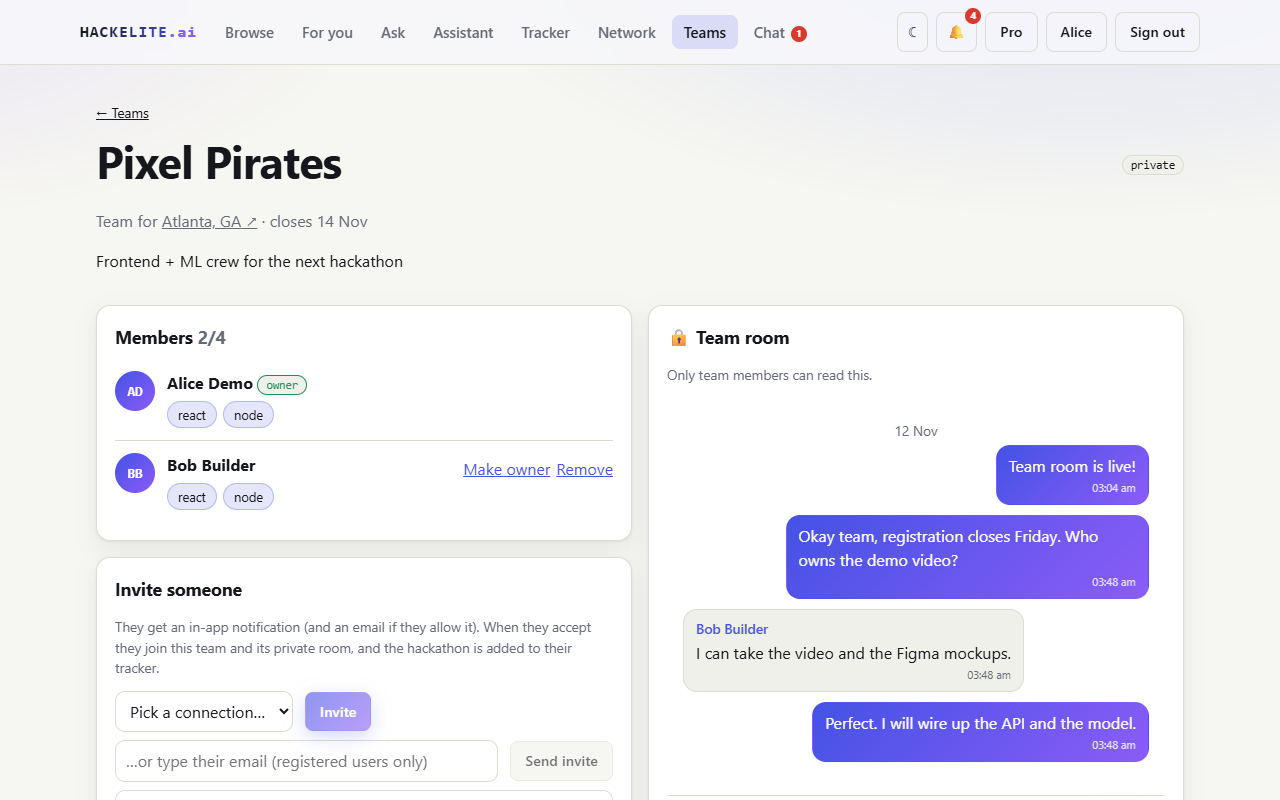
\includegraphics[width=0.92\textwidth]{images/team-room.png}
    \caption{Team Room, Invites and Idea Board}
    \label{fig:team}
\end{figure}

Finally, the interface supports a dark theme and a mobile layout without horizontal scrolling (Figure~\ref{fig:dark} and Figure~\ref{fig:mobile}).

\begin{figure}[H]
    \centering
    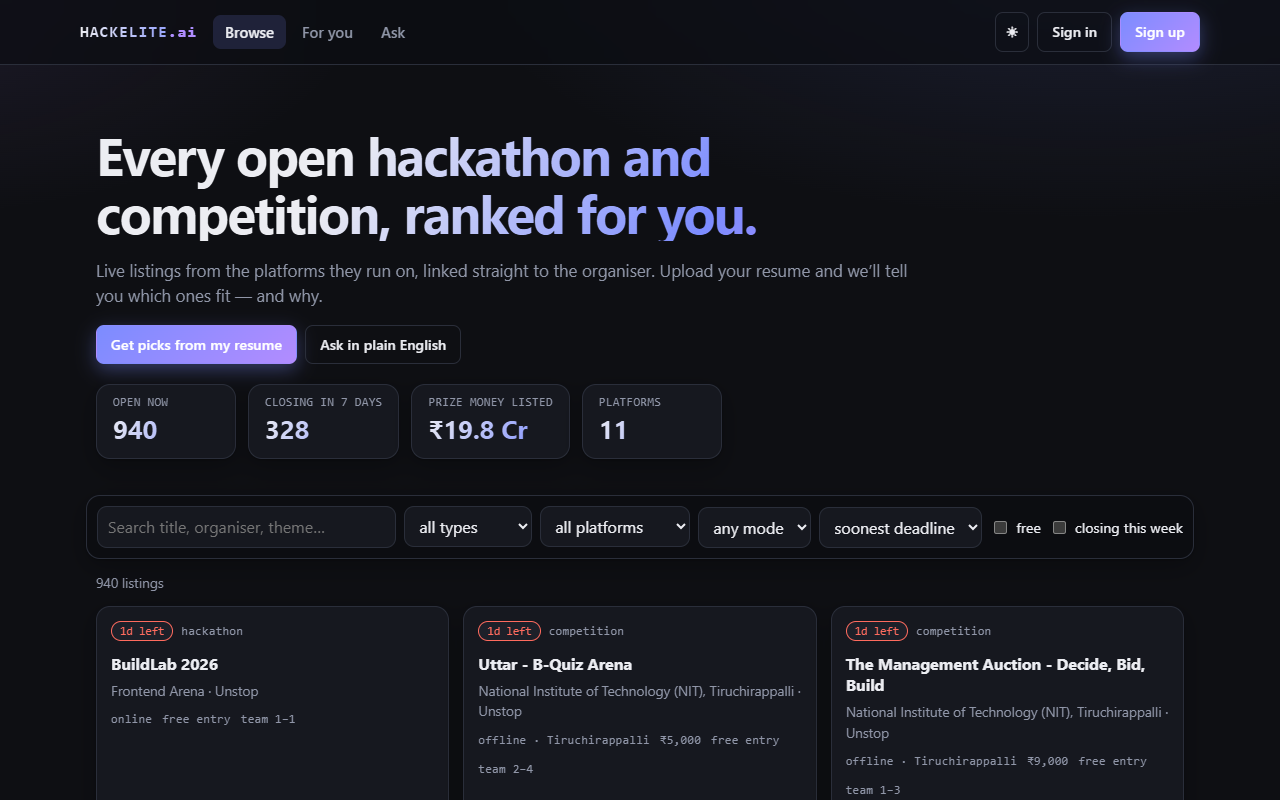
\includegraphics[width=0.92\textwidth]{images/home-dark.png}
    \caption{Dark Theme}
    \label{fig:dark}
\end{figure}

\begin{figure}[H]
    \centering
    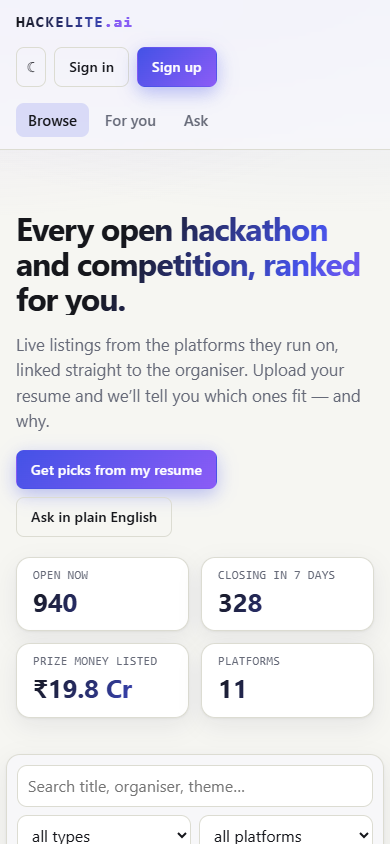
\includegraphics[height=0.45\textheight,keepaspectratio]{images/mobile-home.png}
    \caption{Mobile Layout (390 px width)}
    \label{fig:mobile}
\end{figure}

\subsection{Verification results}
Table~\ref{tab:results} summarises the measured outcomes of the verification run recorded in the project's status document.

\begin{table}[H]
\centering
\caption{Summary of Verification Results}
\label{tab:results}
\begin{tabularx}{\textwidth}{|X|l|}
\hline
\textbf{Check} & \textbf{Result} \\
\hline
Automated server tests (unit, integration, in-process journey) & 114 passing \\
\hline
Live end-to-end journey against a separate server process & 41 of 41 checks passed \\
\hline
Browser click-through journeys in Chromium (optional suite) & 16 of 16 passed \\
\hline
Client production build & Passes, about 103 KB gzipped JavaScript \\
\hline
Dependency audit (server and client, production) & 0 vulnerabilities \\
\hline
Live ingestion & About 940 open listings from 10 sources \\
\hline
Responsive layout & No horizontal scroll at 390 px on browse, login and For you \\
\hline
\end{tabularx}
\end{table}

\section{Testing}
Testing is organised in layers. The \textbf{unit and integration} layer runs the real Express application in process against a real MongoDB and real WebSocket clients, using a throwaway database that each suite creates and drops. The \textbf{in-process journey} runs the whole product story in 11 phases. The \textbf{live end-to-end} runner starts \code{node server.js} as a separate process on a free port with an isolated database, ingestion disabled and mail printed instead of sent, runs the same journey through the public HTTP API and Socket.IO only, and then stops the server and drops the database. The live run is valuable because it catches defects that exist only in a real process: it found a bug in which a valid PDF resume returned HTTP 500 because uploads arrive as a view into a shared network buffer, which in-process tests could not reproduce. The continuous-integration workflow runs the server tests, the live run against a \code{mongo:7} service, the client build, \code{npm audit} and a Docker image build on every push.

\begin{table}[H]
\centering
\caption{Test Cases}
\small
\begin{tabularx}{\textwidth}{|>{\RaggedRight\arraybackslash}p{3.1cm}|X|l|}
\hline
\textbf{Test Case} & \textbf{Description} & \textbf{Status} \\
\hline
Security and API (20) & Headers, CORS, body limits, password policy, register/login/lockout, NoSQL injection, prototype pollution, privilege escalation, reset and verification, plans, resume, assistant, listings, tracker, notifications, lister approval, admin guards, rate limiting, account deletion, privacy isolation, health, breached passwords & Pass \\
\hline
Social (13) & Connections and blocking, live notifications, direct messages over WebSocket, socket authentication attacks, private rooms, teams and invites, Free/Pro split, downgrade grandfathering, join requests, idea voting, reminders, deletion cascade & Pass \\
\hline
Calendar (9) & RFC 5545 folding, escaping, UTC and UIDs, reminders, Google/Outlook links, feed token rotation, revocation and privacy & Pass \\
\hline
Page agent (7) & SSRF guard including IPv4-mapped IPv6, robots.txt, extraction, caching, prompt injection, robots-blocked and private redirects & Pass \\
\hline
Crawler (9) & Same-site discovery, FAQ extraction, PII scrubbing, Crawl-delay, never fetching forum or participant pages, one-second spacing, anonymous tally & Pass \\
\hline
Ingestion pipeline (15) & Dates and time zones, prize parsing, validation reasons, de-duplication, pagination, retries, adapters with stubbed HTTP & Pass \\
\hline
Ingestion persistence (7) & Upsert, stale removal only after complete syncs, saved items kept, failed source removes nothing & Pass \\
\hline
Recommender (10) & Six realistic student profiles, hard exclusions, determinism, free tier, no duplicates & Pass \\
\hline
Resume (10) & Text analysis, real PDF and DOCX fixtures, buffer-view regression, unreadable PDF returns 400 & Pass \\
\hline
Ask and place (2) & Place parsing and hard place filter & Pass \\
\hline
Product journey (1, 11 phases) & Platform, accounts, discovery, plans and recommendations, tracker and calendar, event agent, network and chat, reminders, organiser and admin, privacy sweep, erasure & Pass \\
\hline
Live end-to-end (41 checks) & Same journey against a separately started server process & Pass \\
\hline
\end{tabularx}
\end{table}

The journey's phases are summarised in Table~\ref{tab:journey}. Every step uses only the public HTTP API and Socket.IO, exactly like the browser.

\begin{table}[H]
\centering
\caption{Phases of the Product Journey}
\label{tab:journey}
\small
\begin{tabularx}{\textwidth}{|c|l|X|}
\hline
\textbf{\#} & \textbf{Phase} & \textbf{Highlights} \\
\hline
1 & Platform & Liveness and readiness, security headers, request ids, 404 and 413 \\
\hline
2 & Accounts & Weak password refused, single-use verification link, generic login errors, injection payloads, password change revokes sessions \\
\hline
3 & Discovery & Catalogue, filters, search, sort, expired events hidden, detail \\
\hline
4 & Plans and recommendations & Free gate (402), Pro activation, real PDF parsed (fake refused), deterministic rubric, hard place filter, injection-resistant assistant \\
\hline
5 & Tracker and calendar & Register becomes applied and never downgrades, personalised \code{.ics}, feed token rotate and revoke \\
\hline
6 & Event agent & FAQ crawl with citations, private addresses refused, anonymous tally, private history \\
\hline
7 & Network, chat, teams & Opt-in discovery, live DMs, Free cannot host, Pro hosts and Free invitee joins, idea voting, blocking \\
\hline
8 & Reminders & One email in the window, never twice, only opted-in users \\
\hline
9 & Organiser and admin & Approval, template validation, publish and delete, audit log \\
\hline
10 & Privacy sweep & \code{no-store} on personal routes, secrets never serialised, cross-user isolation \\
\hline
11 & Erasure & Re-authentication required, session revoked, team handed over, DM deleted \\
\hline
\end{tabularx}
\end{table}

\subsection{Defects found and fixed through testing}
Testing found and led to the correction of the following defects: a faulty hand-made PDF fixture (replaced with a real browser-rendered PDF); Devpost short and cross-year date ranges being dropped; a prize written as ``Rs. 50000'' not being parsed; de-duplication wrongly merging different editions of an event with the same name; unparseable dates being reported as missing; an in-person event abroad ranking fourth for a student who does not travel; a matching graduation batch being reported as unknown instead of eligible; the resume page not listing extracted skills; the statistics counting unpublished listings; and the coverage header counting sample listings as ingested.

\subsection{Limitations of the evaluation}
Some components could not be verified against the real third party during development: Google sign-in (verified with a mocked verifier), Gemini generation and embeddings (no key; the extractive mode is tested), SMTP delivery, and the Kaggle and clist adapters (keys required). Load and performance testing used small datasets, and the browser suite was run only in Chromium without a formal accessibility audit. The documentation lists these gaps explicitly together with the commands that verify them on a machine that has the credentials.

% ---------------- Chapter 5 ----------------
\chapter{CONCLUSION AND FUTURE WORK}

\section{Conclusion}
This project designed, implemented and verified HackElite, a full-stack platform that turns the scattered landscape of hackathons and competitions into a single, personalised and explainable experience. A resilient ingestion pipeline aggregates 16 sources into one MongoDB database, isolating failures so that one broken source never blocks the others. A deterministic eight-criterion recommender, backed by a resume analyser and local or Gemini embeddings, ranks events for each student and explains every score. A retrieval-augmented assistant and a per-event agent answer questions with citations, while a polite and SSRF-safe crawler reads the organiser's own pages. The tracker, calendar feed and reminders keep deadlines visible, and the network, teams and chat subsystems let students move from finding an event to forming a team and communicating in real time, with a Free versus Pro split enforced on the server.

Security and privacy were designed in from the start rather than added afterwards: revocable sessions, breached-password checks, injection and SSRF defences, per-user data isolation and complete account erasure are each covered by automated tests. The verification evidence is strong: 114 automated tests, a 41-check live end-to-end journey that runs against a real server process, a clean production build and a dependency audit with zero vulnerabilities. The project demonstrates that a single-database architecture, without a message queue, vector database or cache server, is sufficient to provide explainable personalisation, retrieval-augmented question answering and real-time collaboration in one product, and that it can be deployed reproducibly with Docker and a continuous-integration pipeline.

\section{Future Work}
\begin{itemize}[leftmargin=*]
    \item Integrate a payment provider and replace activation keys with a webhook that sets the plan tier.
    \item Add chat moderation: reporting, deletion, editing and an administrator review queue.
    \item Separate background jobs into a worker with a queue, add the Socket.IO Redis adapter and a shared rate-limit store, and add leader election to support several API instances.
    \item Adopt MongoDB Atlas Vector Search for similarity queries as the catalogue and the number of users grow.
    \item Use a headless browser for event pages that render only with JavaScript, while continuing to respect robots.txt and terms of service.
    \item Move the session token to an httpOnly SameSite cookie with CSRF protection, add refresh tokens, and require email verification for organisers and Pro users.
    \item Build a native mobile application with push notifications and extend the progressive web app support.
    \item Add model-based skill extraction in place of the dictionary, per-university adapters, official partner APIs, and a formal accessibility (WCAG) audit.
    \item Add observability: metrics, alerting and centralised log shipping.
\end{itemize}

% ---------------- References ----------------
\clearpage
\addcontentsline{toc}{chapter}{References}

\begin{thebibliography}{00}

\bibitem{ref1}
P. Lewis \emph{et al.}, ``Retrieval-augmented generation for knowledge-intensive NLP tasks,'' in \emph{Advances in Neural Information Processing Systems (NeurIPS)}, vol. 33, 2020.

\bibitem{ref2}
K. Weinberger, A. Dasgupta, J. Langford, A. Smola, and J. Attenberg, ``Feature hashing for large scale multitask learning,'' in \emph{Proc. 26th International Conference on Machine Learning (ICML)}, 2009.

\bibitem{ref3}
N. Provos and D. Mazi{\`e}res, ``A future-adaptable password scheme,'' in \emph{Proc. USENIX Annual Technical Conference}, 1999.

\bibitem{ref4}
M. Jones, J. Bradley, and N. Sakimura, ``JSON Web Token (JWT),'' RFC 7519, Internet Engineering Task Force, 2015.

\bibitem{ref5}
I. Fette and A. Melnikov, ``The WebSocket protocol,'' RFC 6455, Internet Engineering Task Force, 2011.

\bibitem{ref6}
B. Desruisseaux, Ed., ``Internet calendaring and scheduling core object specification (iCalendar),'' RFC 5545, Internet Engineering Task Force, 2009.

\bibitem{ref7}
M. Koster, G. Illyes, H. Zeller, and L. Sassman, ``Robots exclusion protocol,'' RFC 9309, Internet Engineering Task Force, 2022.

\bibitem{ref8}
OWASP Foundation, ``OWASP Top Ten 2021,'' and ``Server-Side Request Forgery Prevention Cheat Sheet.'' [Online]. Available: https://owasp.org

\bibitem{ref9}
T. Hunt, ``Pwned Passwords API v3 and k-anonymity,'' Have I Been Pwned. [Online]. Available: https://haveibeenpwned.com/API/v3

\bibitem{ref10}
MongoDB, Inc., ``MongoDB manual'' and ``Mongoose documentation.'' [Online]. Available: https://www.mongodb.com/docs

\bibitem{ref11}
Express.js, ``Express - Node.js web application framework.'' [Online]. Available: https://expressjs.com

\bibitem{ref12}
Meta Platforms, Inc., ``React documentation'' and Vite, ``Vite documentation.'' [Online]. Available: https://react.dev and https://vite.dev

\bibitem{ref13}
Socket.IO, ``Socket.IO documentation.'' [Online]. Available: https://socket.io/docs

\bibitem{ref14}
OpenJS Foundation, ``Node.js documentation, including the \code{node:test} runner.'' [Online]. Available: https://nodejs.org/docs

\bibitem{ref15}
Google, ``Gemini API documentation: text generation and embeddings.'' [Online]. Available: https://ai.google.dev

\bibitem{ref16}
Docker, Inc., ``Docker documentation'' and GitHub, ``GitHub Actions documentation.'' [Online]. Available: https://docs.docker.com and https://docs.github.com/actions

\bibitem{ref17}
HackElite project repository and documentation (README, ARCHITECTURE, SECURITY, TESTING, SOCIAL, CRAWLER and DEPLOYMENT guides), 2026.

\end{thebibliography}

\end{document}
